
\section{Flujo sobre el dispositivo objetivo}

La simulación funcional permite comprobar el comportamiento del RTL, pero no
muestra cómo se utiliza el dispositivo físico. Para obtener esa información, el
diseño se sintetizó y se implementó sobre la FPGA Artix-7
\texttt{xc7a35tcpg236-1} de la Basys 3.

Durante la síntesis, Vivado interpreta los módulos SystemVerilog y los traduce a
una red formada por registros, memorias, operadores y máquinas de estado. La
implementación toma esa red y asigna cada recurso a una ubicación concreta del
dispositivo. En esta etapa también realiza la colocación, el ruteo y el cálculo
de los retardos físicos. Una vez completadas ambas etapas, se genera el
bitstream utilizado para programar la placa.

El proceso se automatizó mediante dos archivos. El script
\texttt{scripts/create\_project.tcl} crea el proyecto para el dispositivo
seleccionado. También agrega las diez fuentes RTL, los ocho bancos de pruebas y
el archivo de restricciones \texttt{basys3.xdc}. Finalmente, establece
\texttt{alu\_uart\_top} como módulo superior.

El script \texttt{scripts/build\_bitstream.tcl} ejecuta la construcción del
diseño. Primero reinicia las corridas anteriores y vuelve a realizar la
síntesis y la implementación. Luego guarda en el directorio
\texttt{reports/} los reportes de utilización, metodología, temporización, CDC
y DRC. El mismo script genera el archivo
\texttt{build/alu\_uart\_top.bit}.

La creación del proyecto y la construcción completa pueden repetirse con los
siguientes comandos:

\begin{codebox}
	 vivado -mode batch -source scripts/create_project.tcl
	 vivado -mode batch -source scripts/build_bitstream.tcl
\end{codebox}

La construcción utilizada para este informe se realizó con Vivado 2025.2, build
6299465. La síntesis terminó sin errores, advertencias críticas ni advertencias.
Durante la implementación, el ruteo finalizó con el mensaje
\texttt{Router Completed Successfully}. La figura~\ref{fig:corridas-vivado}
muestra el estado final de ambas corridas.

\begin{figure}[H]
	\centering
	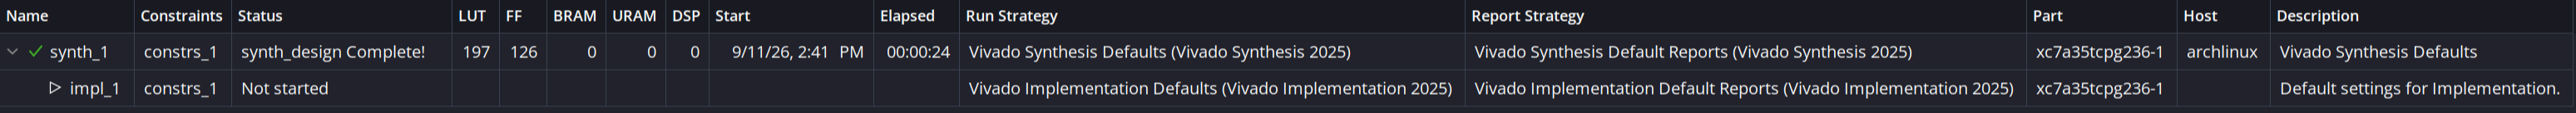
\includegraphics[width=\textwidth,trim=0 0 2347 0,clip]
	{img/vivado_synthesis_successful.png}
	\vspace{0.5em}

	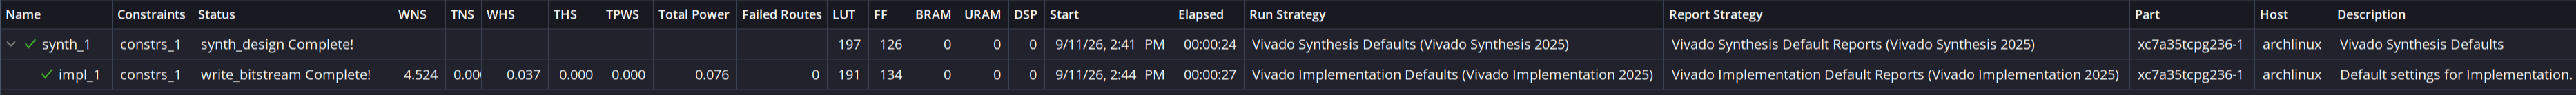
\includegraphics[width=\textwidth,trim=0 0 2500 0,clip]
	{img/vivado_implementation_successful.png}
	\caption{Corridas de síntesis e implementación completadas en Vivado.}%
	\label{fig:corridas-vivado}
\end{figure}

El bitstream obtenido corresponde al dispositivo declarado y ocupa 326538
bytes. La figura~\ref{fig:flujo-vivado} resume el recorrido desde las fuentes
SystemVerilog hasta ese archivo. Los resultados de utilización, temporización,
CDC y DRC se producen durante las etapas intermedias y se analizan por separado
en las secciones siguientes.

\begin{figure}[H]
	\centering
	\begin{tikzpicture}[
			stage/.style={draw=coderule,fill=codeback,rounded corners=2mm,
			minimum width=3.0cm,minimum height=1.35cm,align=center,thick},
			ok/.style={font=\small\bfseries,text=technicalviolet},
			arrow/.style={-{Latex[length=2.4mm]},thick,draw=codeviolet}
		]
		\node[stage] at (0,0) (rtl) {SystemVerilog\\10 módulos};
		\node[stage] at (4.1,0) (synth) {Síntesis\\0 errores};
		\node[stage] at (8.2,0) (place) {Place \& route\\completado};
		\node[stage] at (12.3,0) (bit) {Bitstream\\326538 bytes};
		\draw[arrow] (rtl) -- (synth);
		\draw[arrow] (synth) -- (place);
		\draw[arrow] (place) -- (bit);
		\node[ok,below=0.3cm of synth] {FSM y LUTRAM extraídas};
		\node[ok,below=0.3cm of place] {timing, CDC y DRC};
	\end{tikzpicture}
	\caption{Recorrido reproducido desde RTL hasta el bitstream.}%
	\label{fig:flujo-vivado}
\end{figure}

\section{Elaboración y comprobación del RTL}

Antes de traducir el diseño a los recursos de la FPGA, Vivado elabora las fuentes
y construye su jerarquía lógica. Esta etapa permite comprobar que los módulos,
las instancias y sus conexiones fueron interpretados de acuerdo con la
descripción SystemVerilog.

La figura~\ref{fig:sources-vivado} muestra las fuentes incorporadas al
proyecto. Allí se reconoce el archivo
\texttt{rtl/alu\allowbreak\_uart\allowbreak\_top.sv} como
nivel superior, junto con sus instancias sintetizables. También aparecen
\texttt{basys3.xdc} y los ocho bancos utilizados durante la simulación.

\begin{figure}[H]
	\centering
	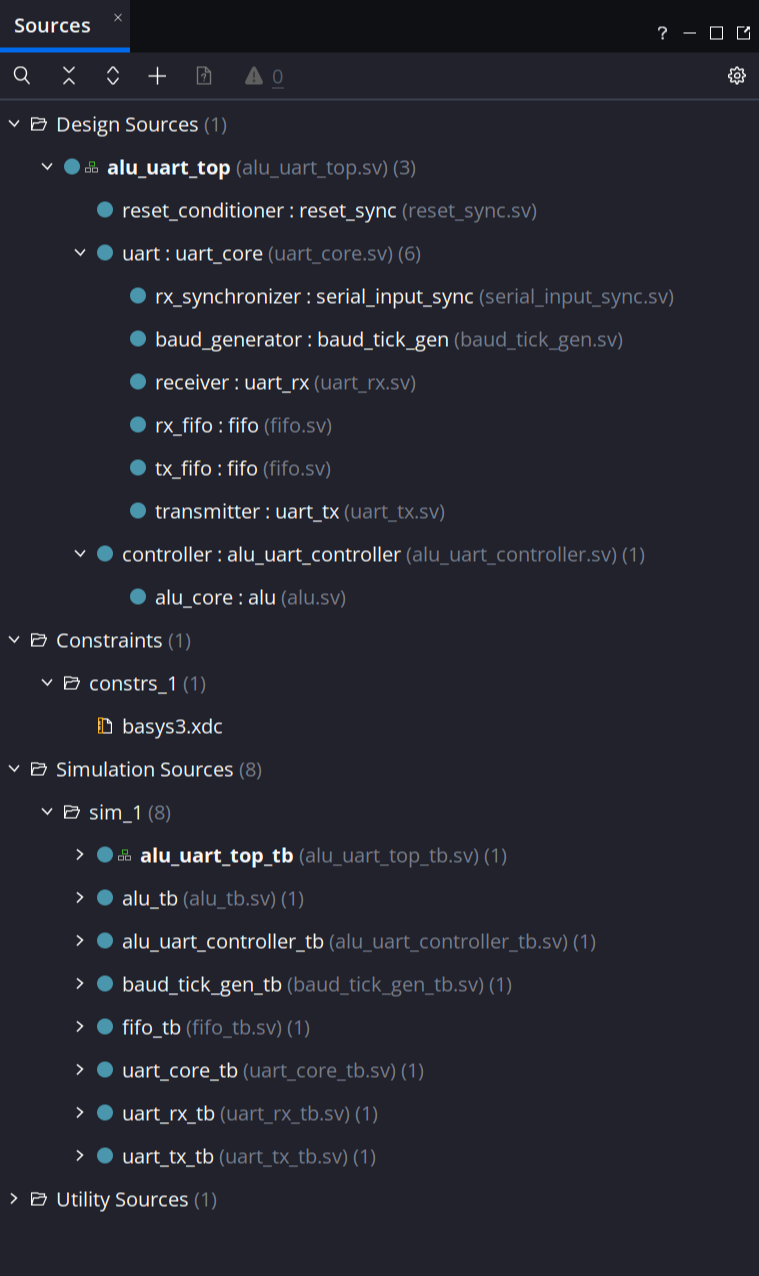
\includegraphics[height=14.2cm,keepaspectratio]{img/vivado_sources.png}
	\caption{Jerarquía de fuentes, restricciones y bancos de pruebas en Vivado.}%
	\label{fig:sources-vivado}
\end{figure}

Sobre esta misma configuración se ejecutó el análisis estático del RTL. La
herramienta revisó la descripción antes de la síntesis y no encontró
violaciones. El resultado se observa en la
figura~\ref{fig:linter-vivado}.

\begin{figure}[H]
	\centering
	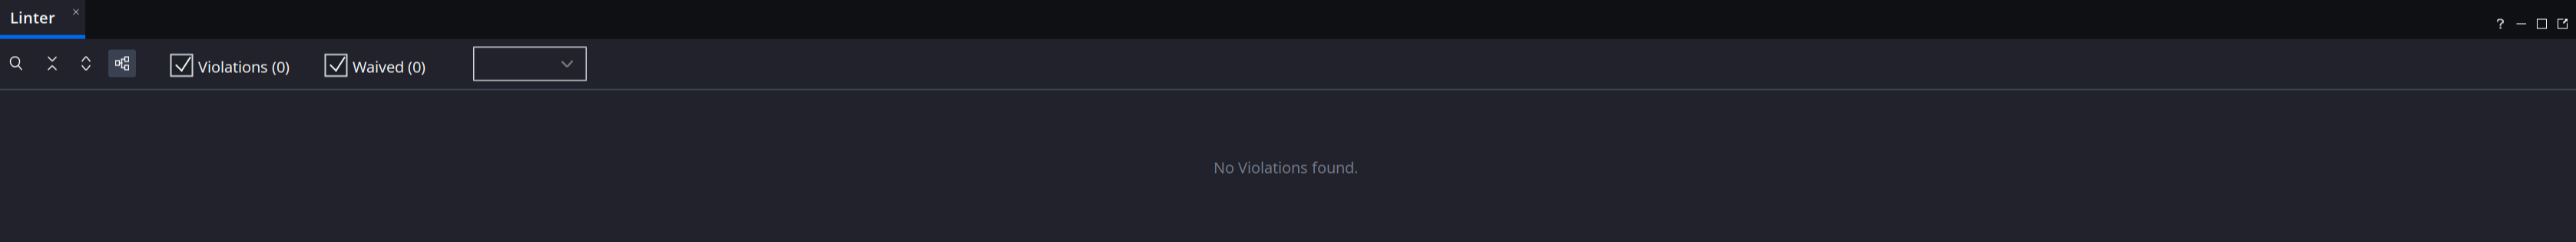
\includegraphics[width=\textwidth]{img/vivado_linter.png}
	\caption{Análisis estático del RTL sin violaciones.}%
	\label{fig:linter-vivado}
\end{figure}

Los esquemáticos elaborados permiten revisar la estructura que Vivado obtuvo a
partir de las fuentes. En esta vista todavía se conservan los módulos del RTL.
Por lo tanto, resulta posible comparar directamente la jerarquía generada con la
arquitectura presentada anteriormente.

La revisión comienza en el nivel superior. En la
figura~\ref{fig:schematic-top-rtl} se distinguen el acondicionador del reset, el
núcleo UART y el controlador de las transacciones. Estos bloques se mantienen
separados y se conectan mediante las señales definidas en
\texttt{rtl/alu\_uart\_top.sv}.

\begin{figure}[H]
	\centering
	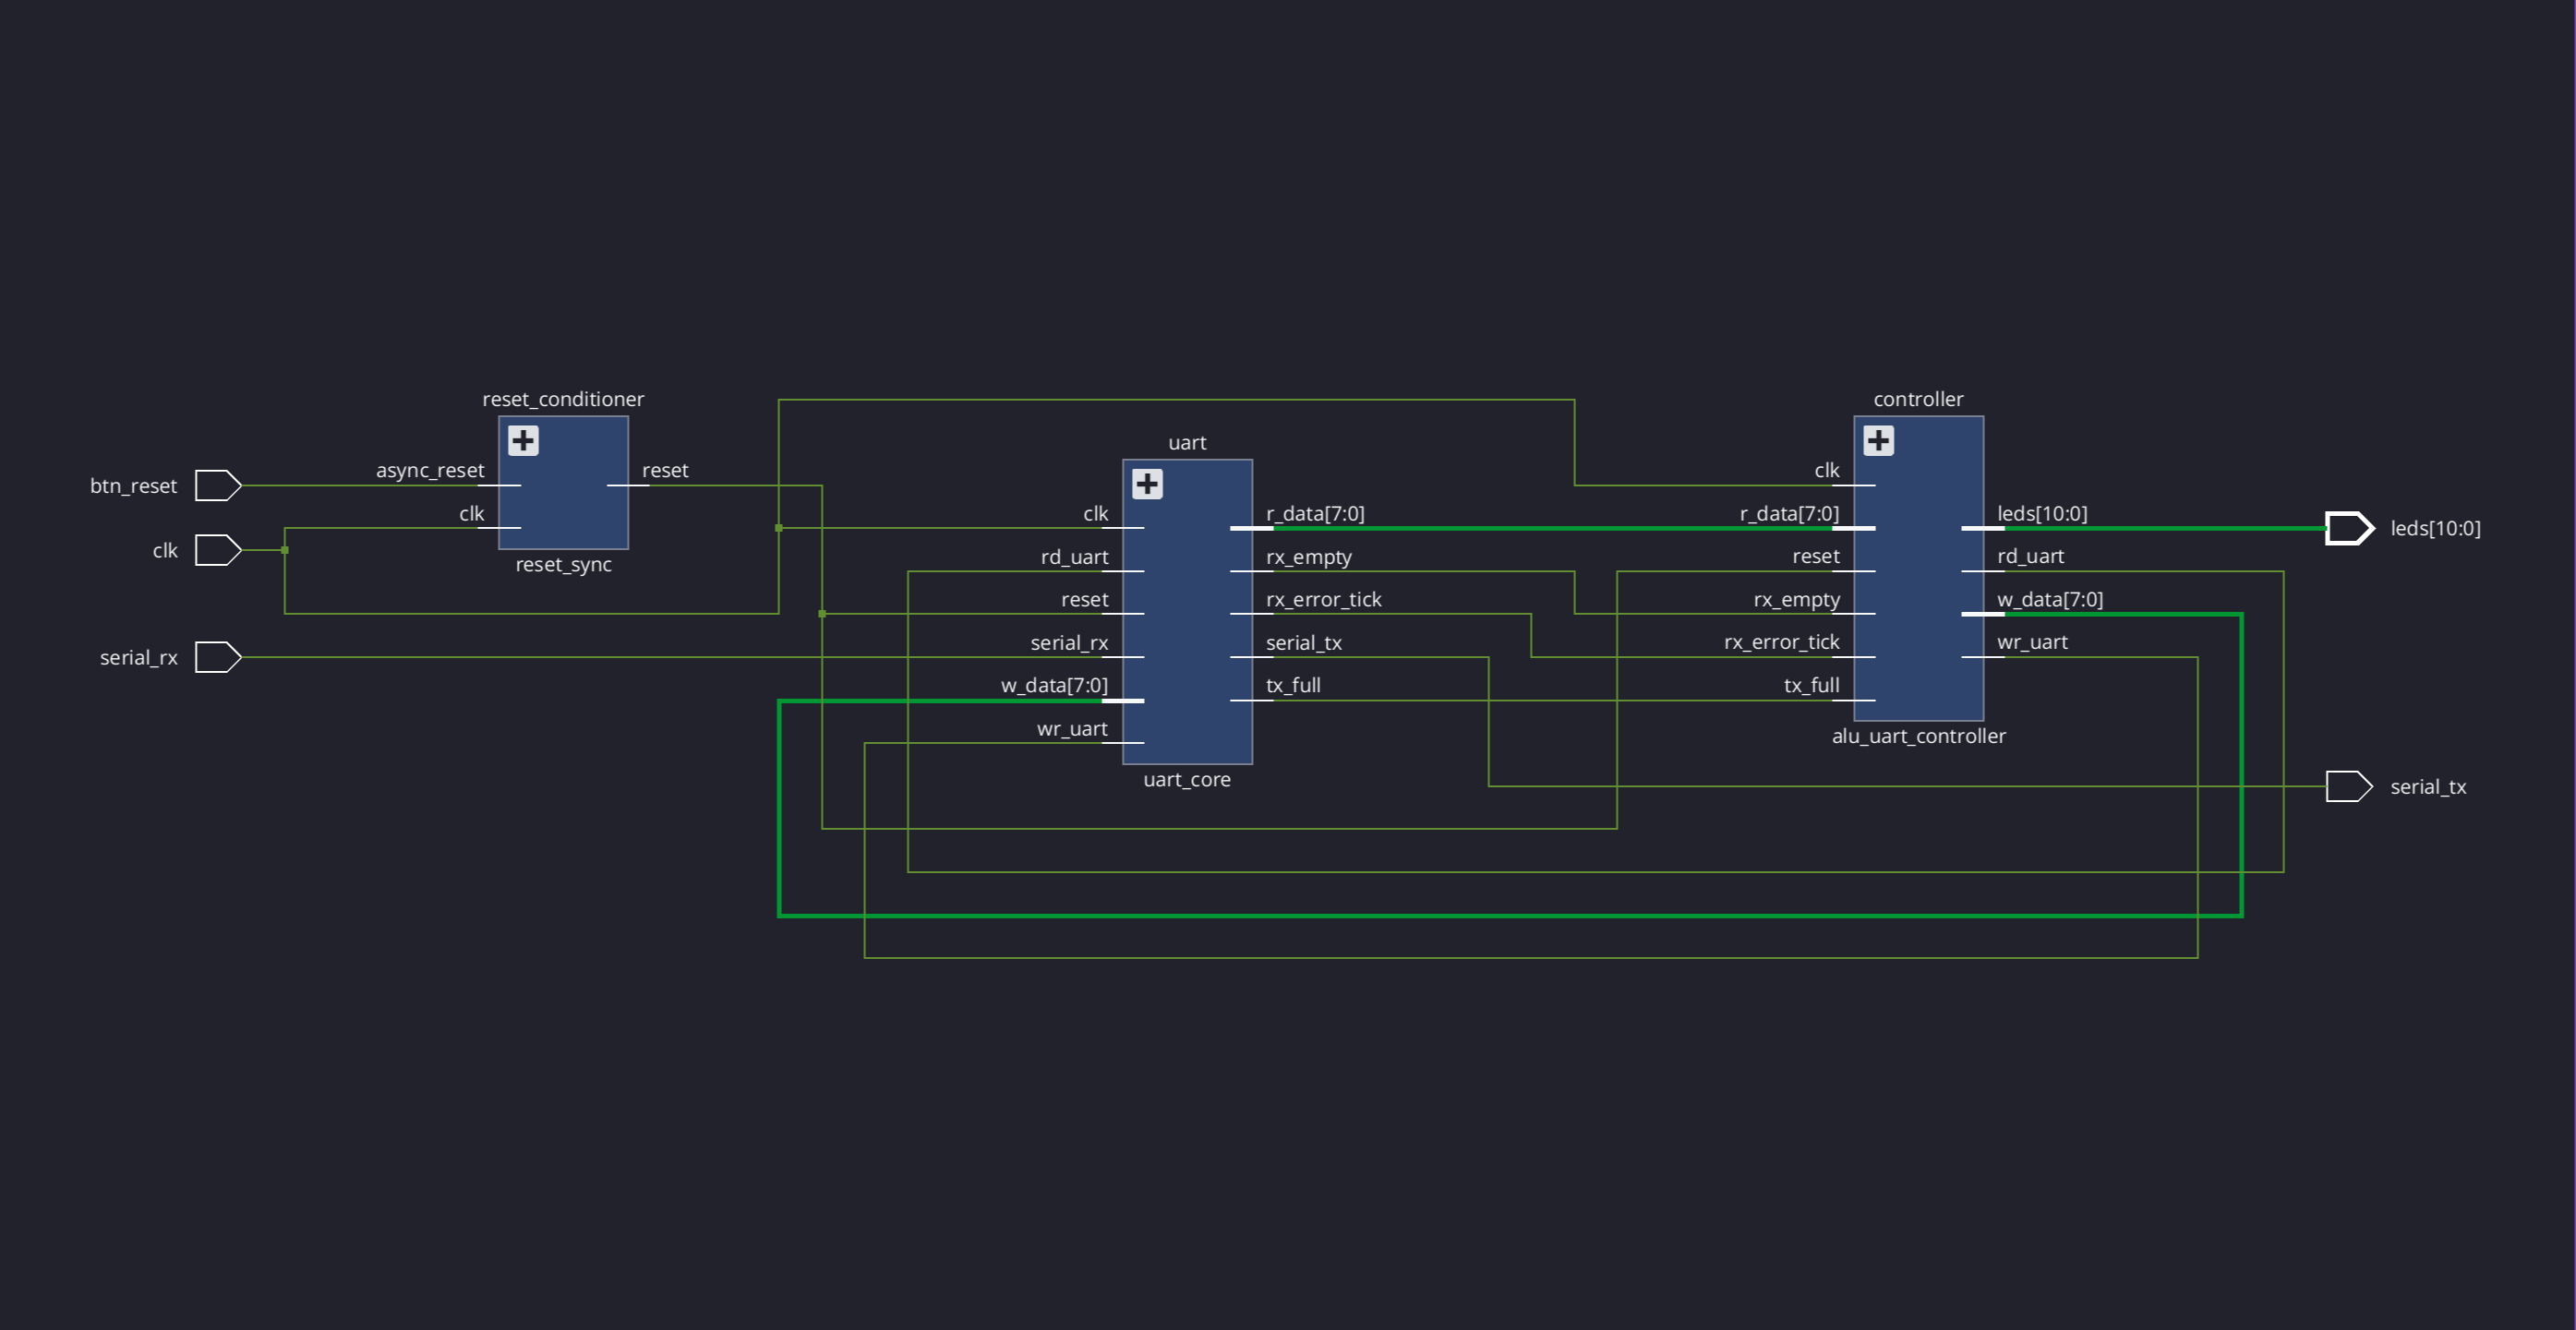
\includegraphics[width=0.92\textwidth]{img/vivado_schematic_top_rtl.png}
	\caption{Esquemático RTL elaborado de \texttt{alu\_uart\_top}.}%
	\label{fig:schematic-top-rtl}
\end{figure}

Al ingresar en el núcleo UART se observan los dos caminos de la comunicación.
La figura~\ref{fig:schematic-uart-core-rtl} muestra el receptor con su FIFO y
el transmisor con la cola de salida. Ambos caminos utilizan el mismo generador
de muestreo. Esta organización coincide con la descripción del archivo
\texttt{rtl/uart\_core.sv}.

\begin{figure}[H]
	\centering
	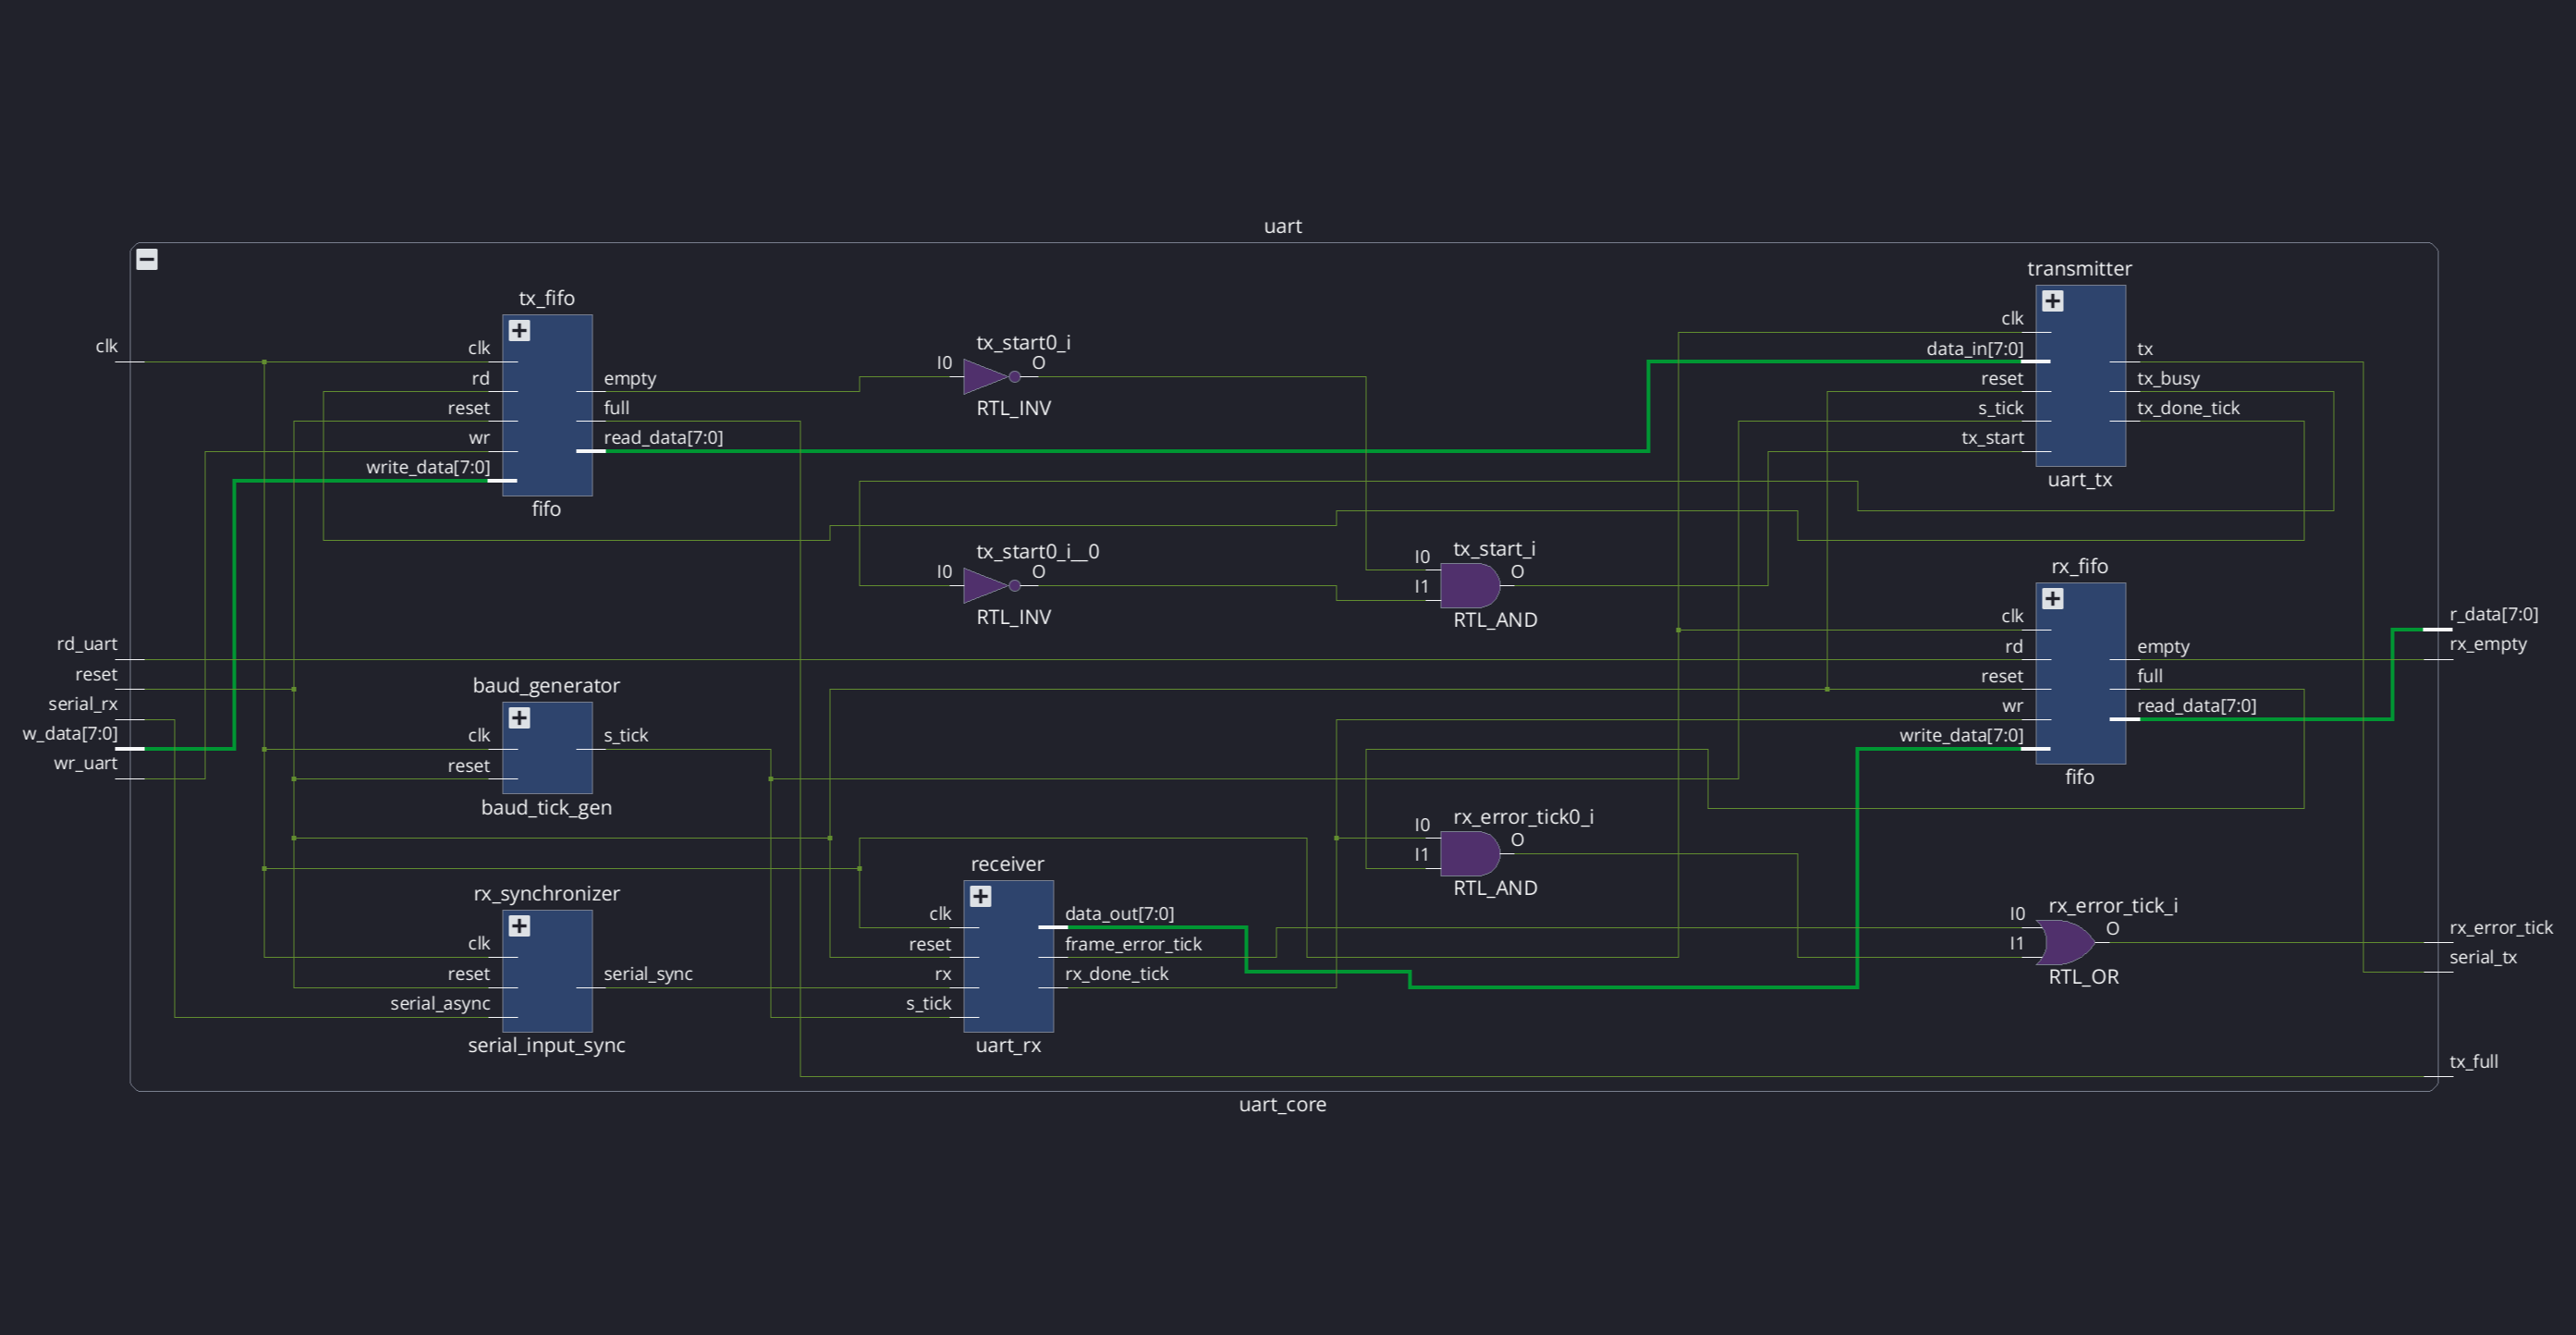
\includegraphics[width=0.92\textwidth]{img/vivado_schematic_uart_core_rtl.png}
	\caption{Esquemático RTL elaborado de \texttt{uart\_core}.}%
	\label{fig:schematic-uart-core-rtl}
\end{figure}

Los circuitos que preparan las señales de entrada se revisaron por separado. La
figura~\ref{fig:schematics-conditioning-rtl} reúne el acondicionador del reset,
el sincronizador de \texttt{serial\_rx} y el generador de
\texttt{s\_tick}. Los esquemáticos confirman que estas funciones permanecen
en módulos independientes antes de conectarse con el resto del sistema.

\begin{figure}[H]
	\centering
	\begin{minipage}[t]{0.49\textwidth}
		\centering
		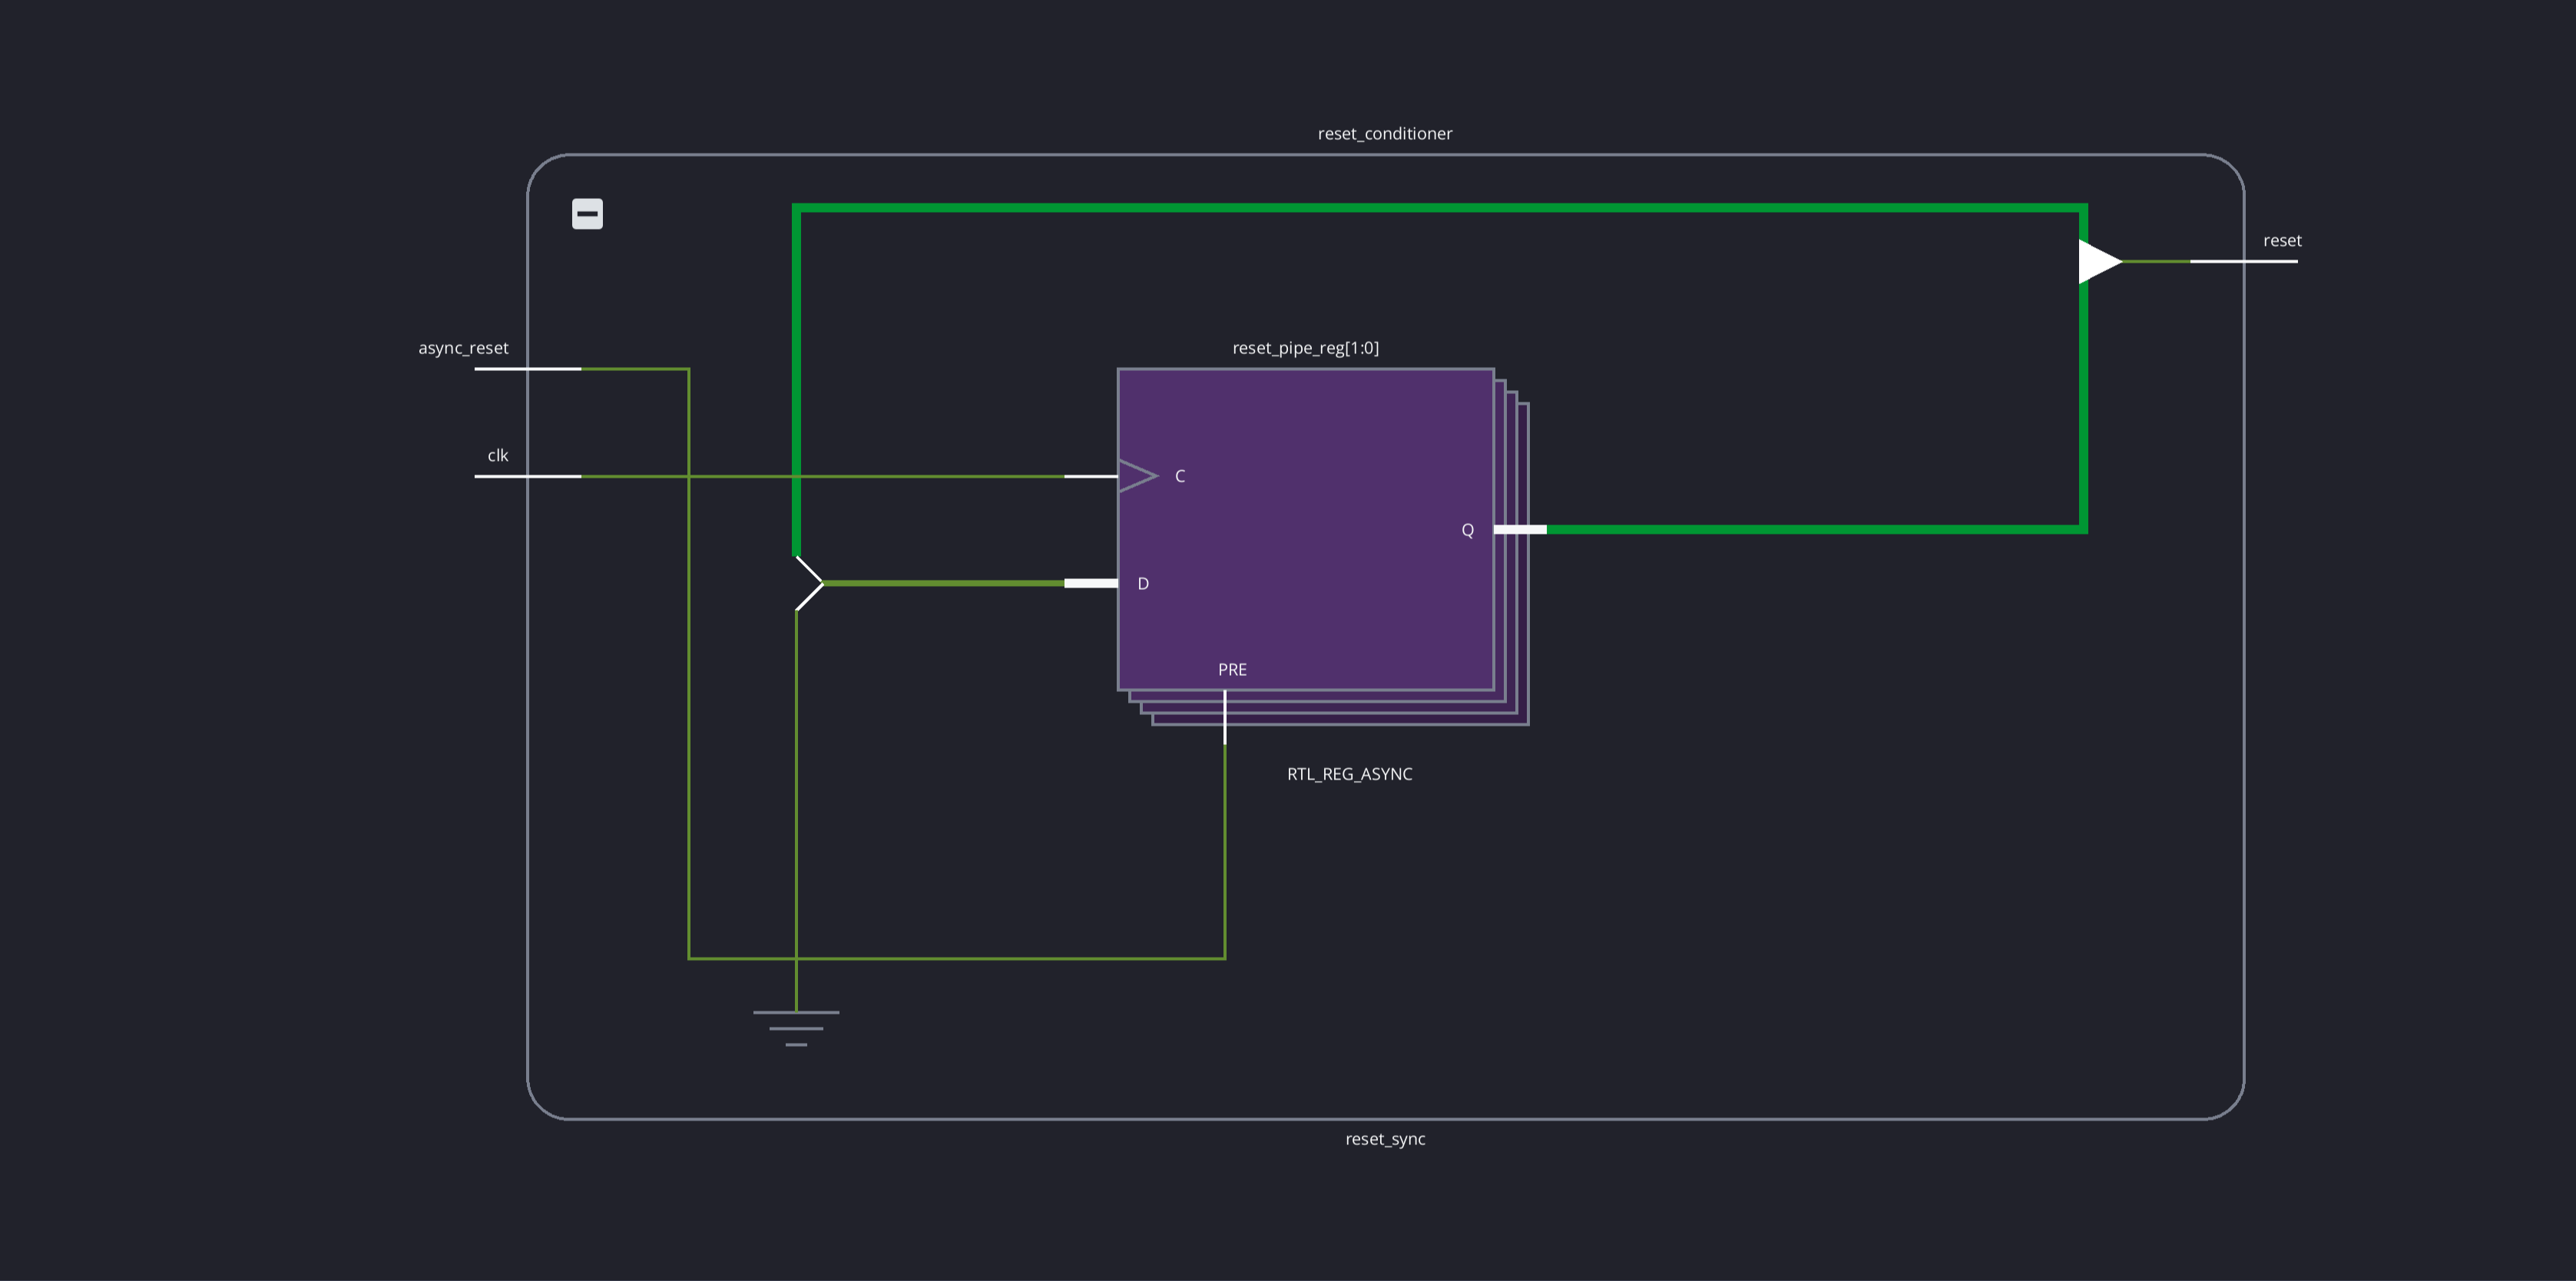
\includegraphics[width=\linewidth]{img/vivado_schematic_reset_sync_rtl.png}
	\end{minipage}\hfill
	\begin{minipage}[t]{0.49\textwidth}
		\centering
		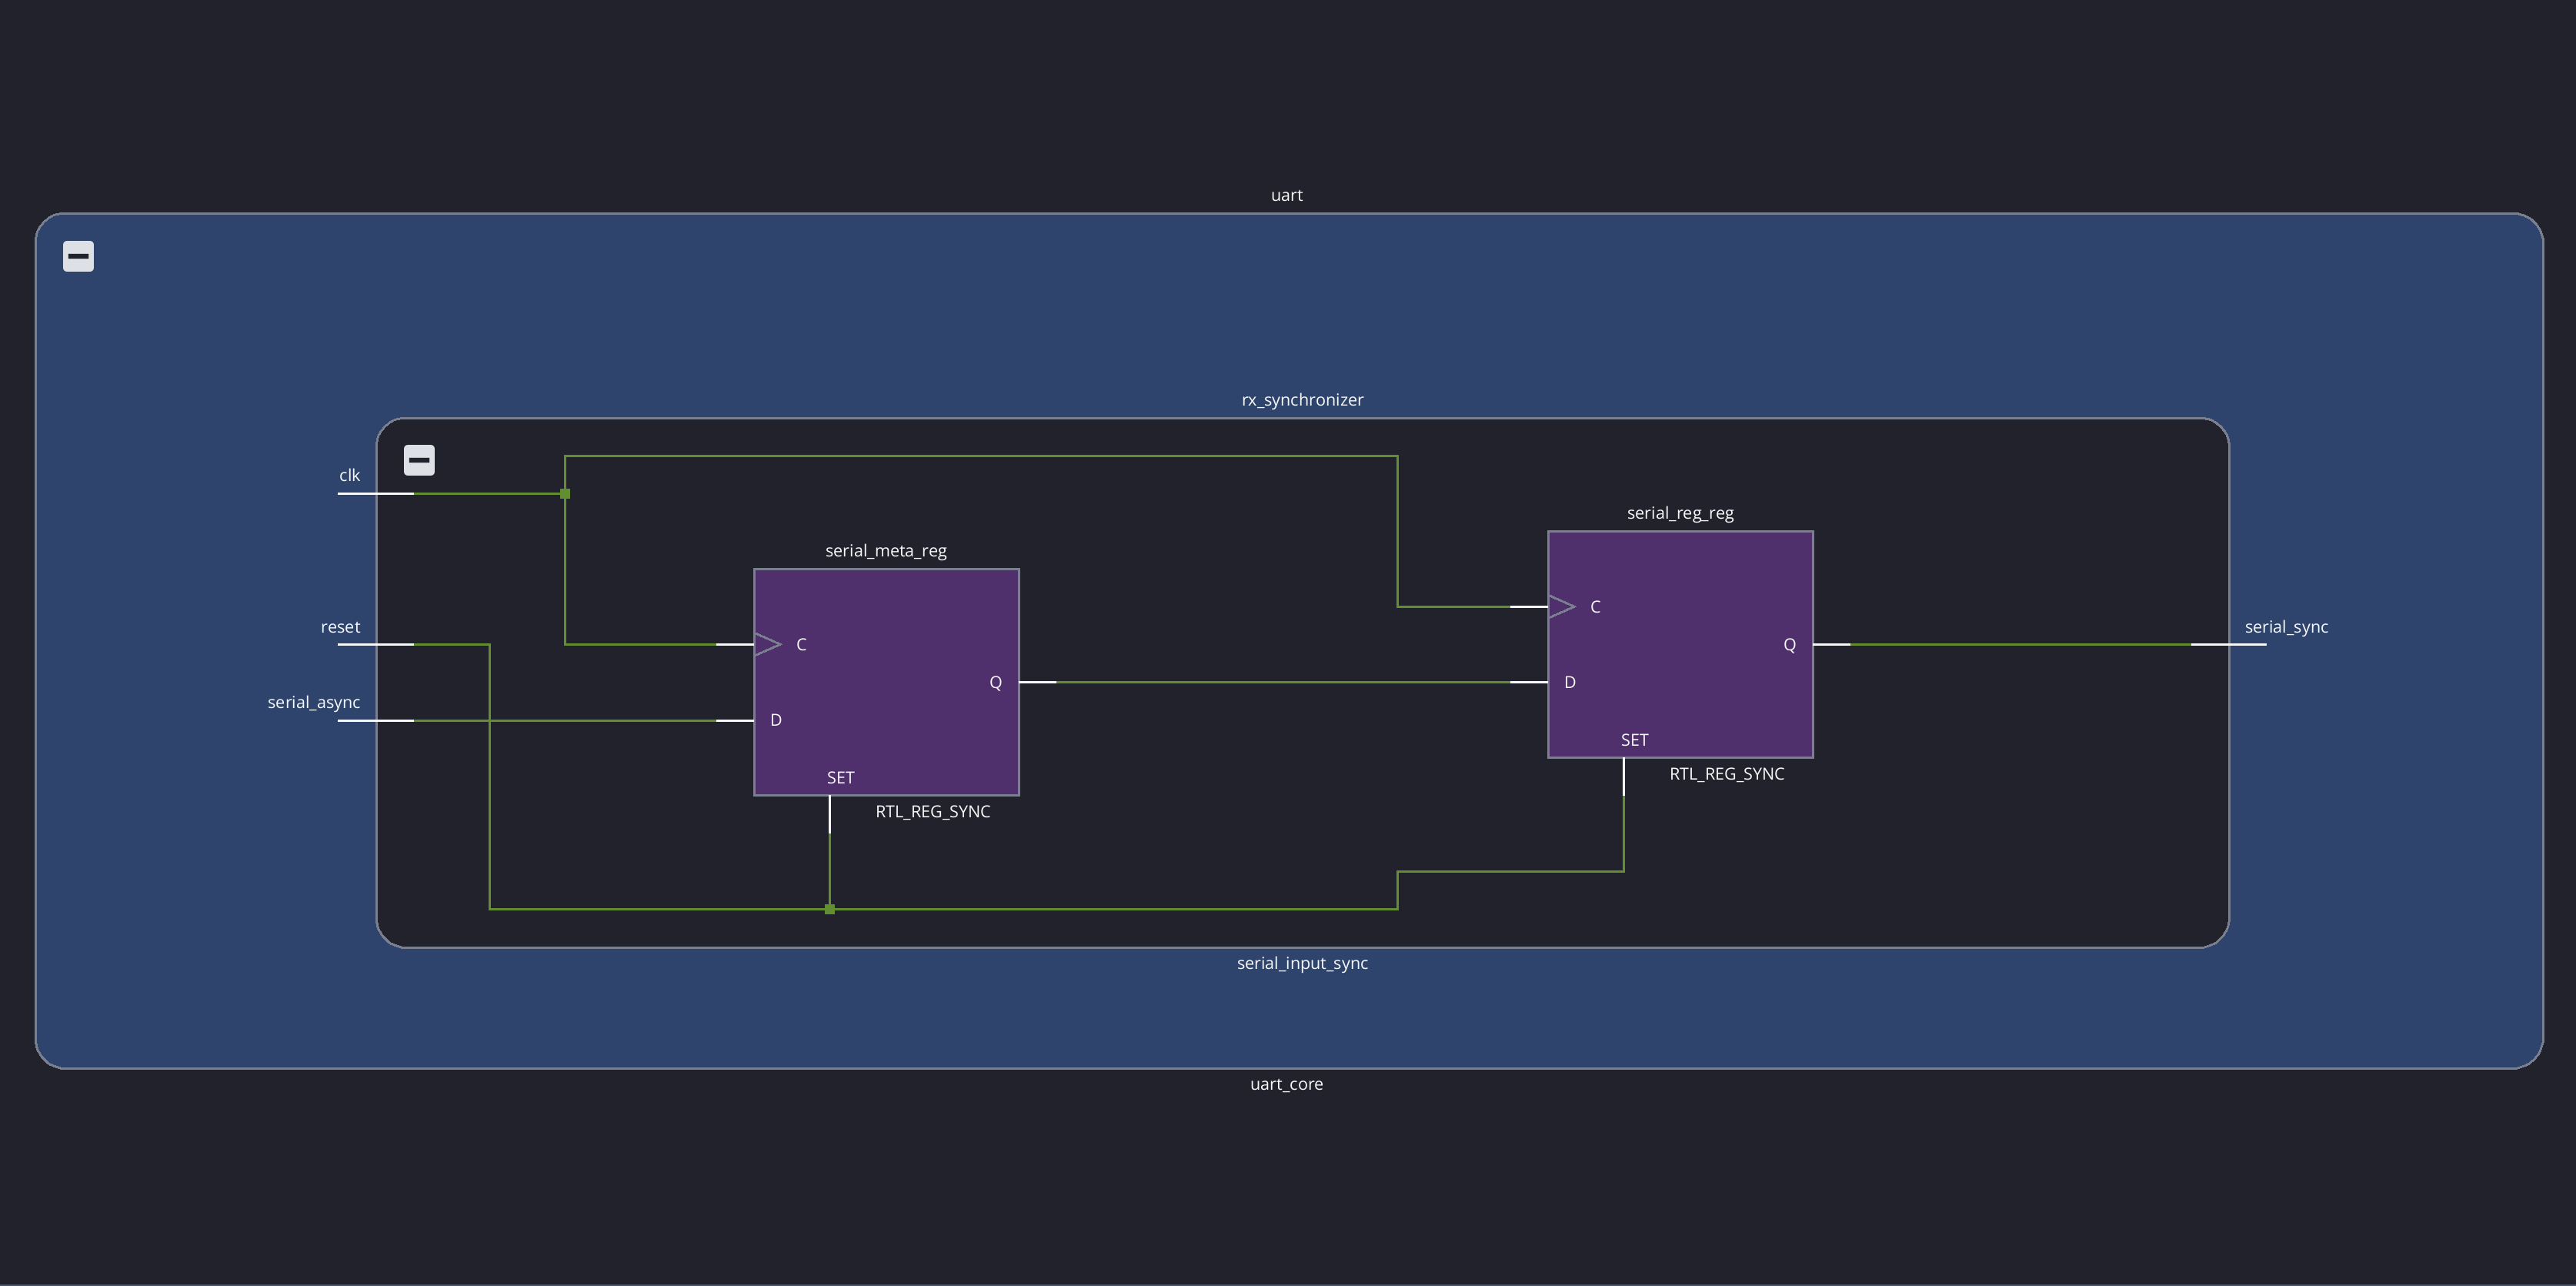
\includegraphics[width=\linewidth]{img/vivado_schematic_serial_input_sync_rtl.png}
	\end{minipage}
	\vspace{0.6em}

	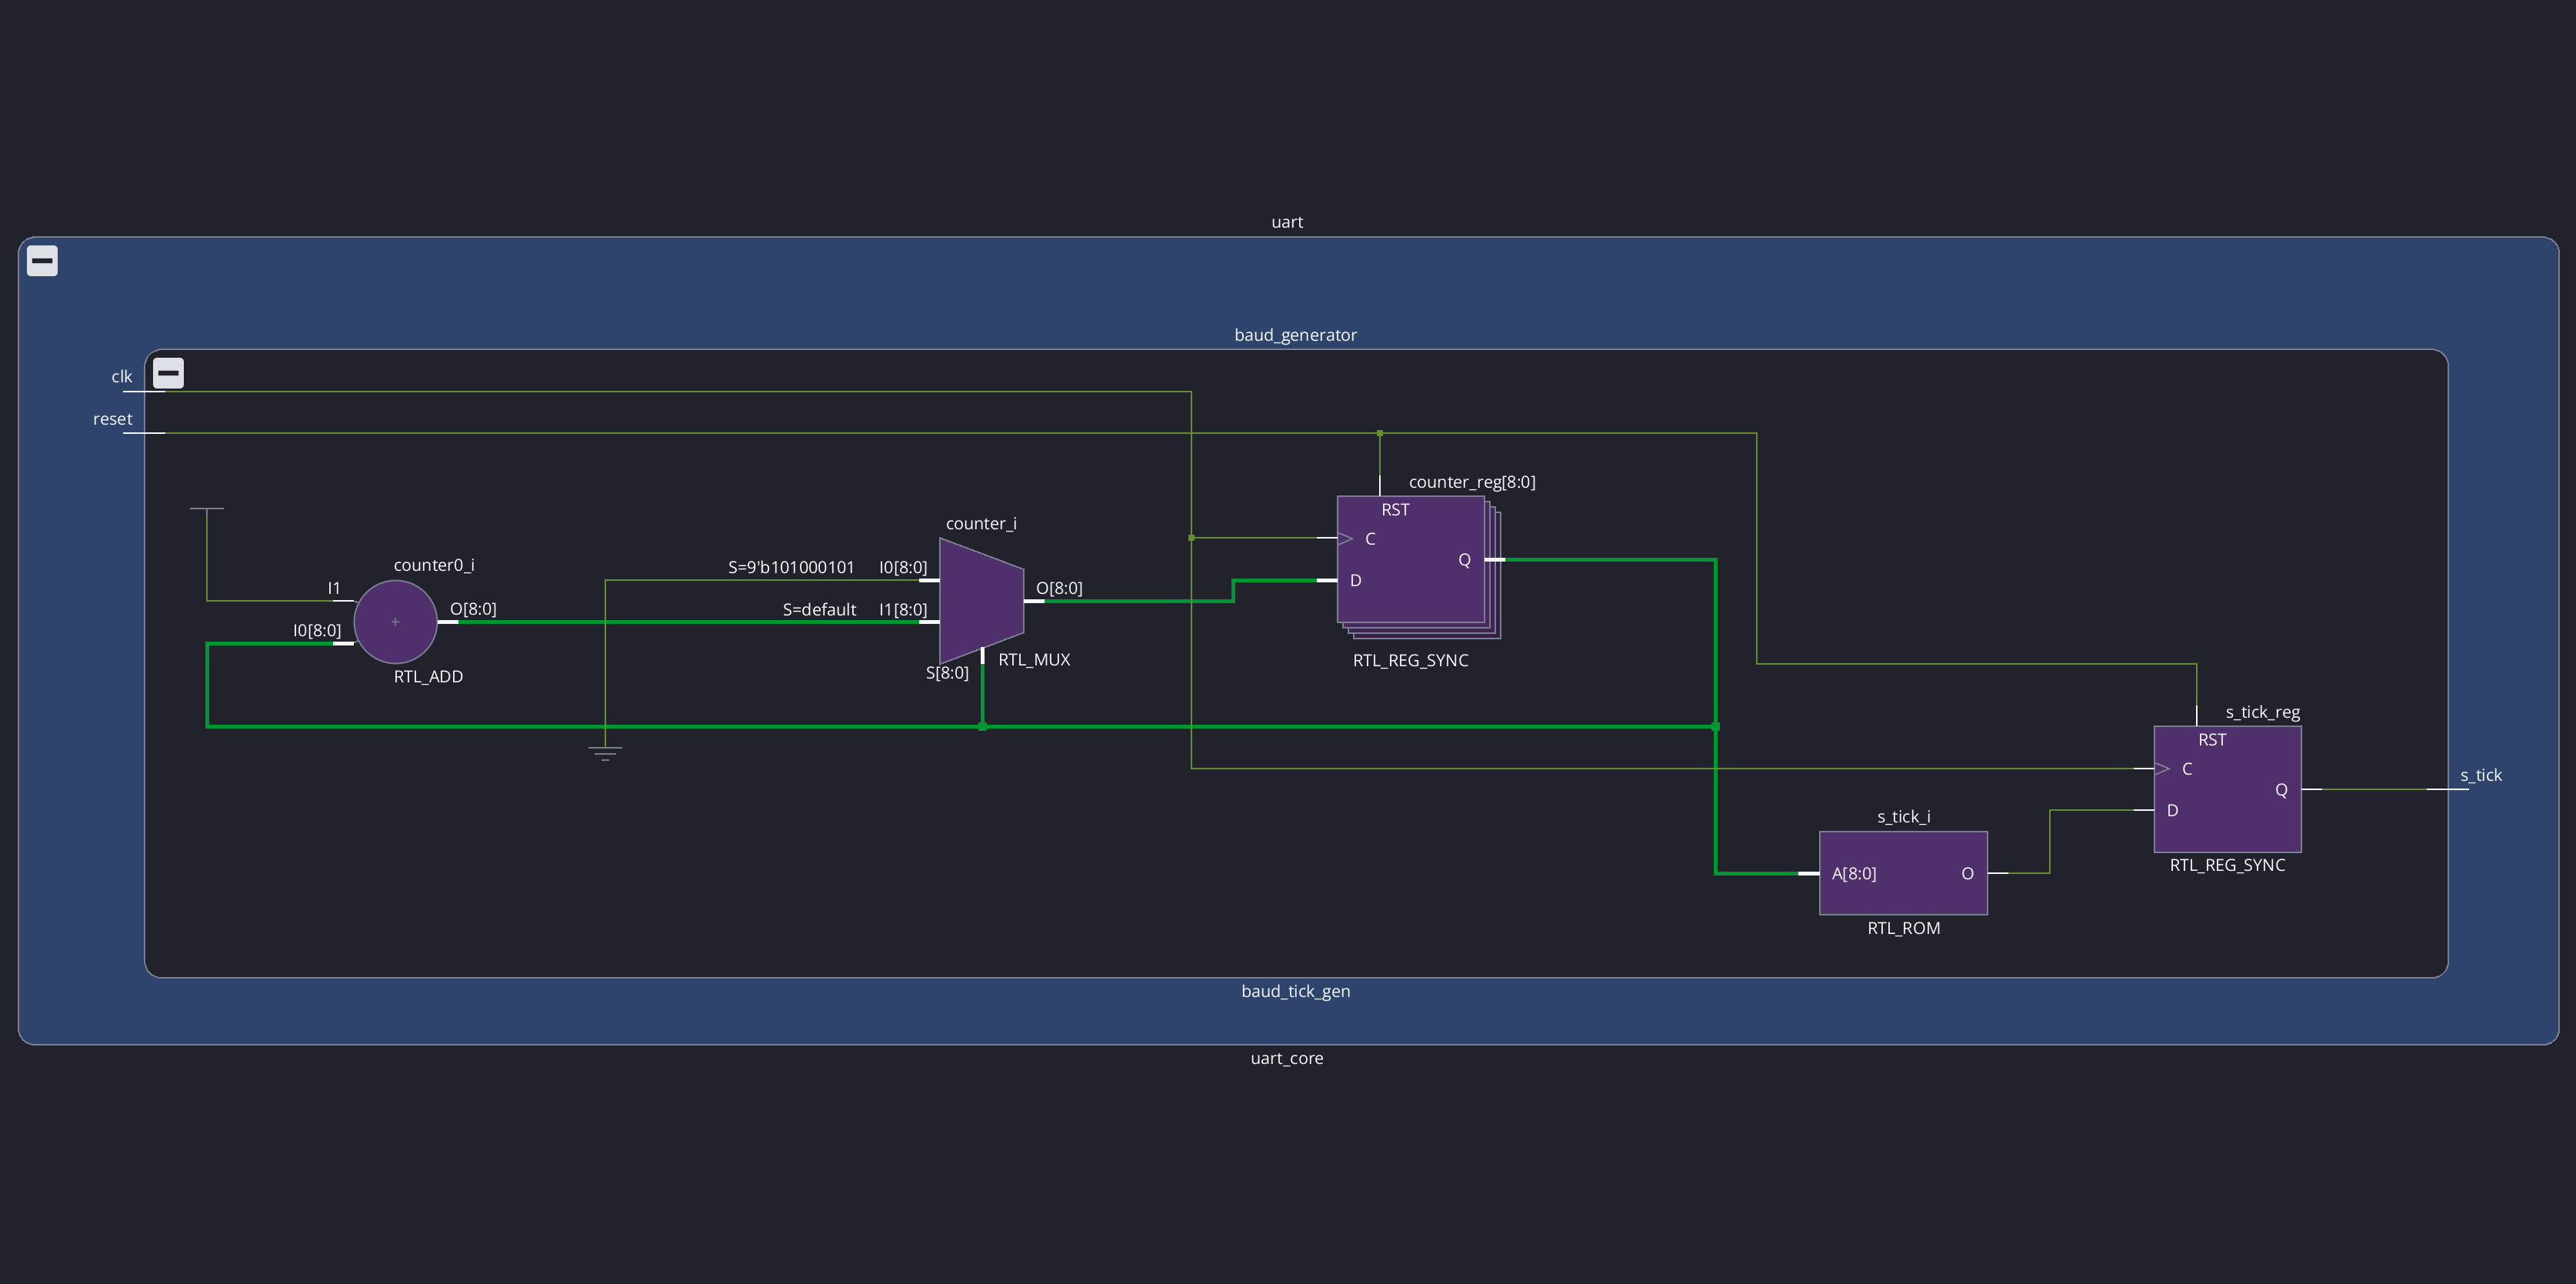
\includegraphics[width=0.72\textwidth]{img/vivado_schematic_baud_tick_gen_rtl.png}
	\caption{Esquemáticos RTL del acondicionamiento de reset, el sincronizador de
	entrada y el generador de muestreo.}%
	\label{fig:schematics-conditioning-rtl}
\end{figure}

La figura~\ref{fig:schematics-rx-tx-rtl} presenta los dos módulos que forman y
reconstruyen las tramas. El esquemático de \texttt{uart\_rx} corresponde al
camino que convierte la entrada serie en un byte. El de \texttt{uart\_tx}
muestra el recorrido inverso desde un byte hasta la salida serie.

\begin{figure}[H]
	\centering
	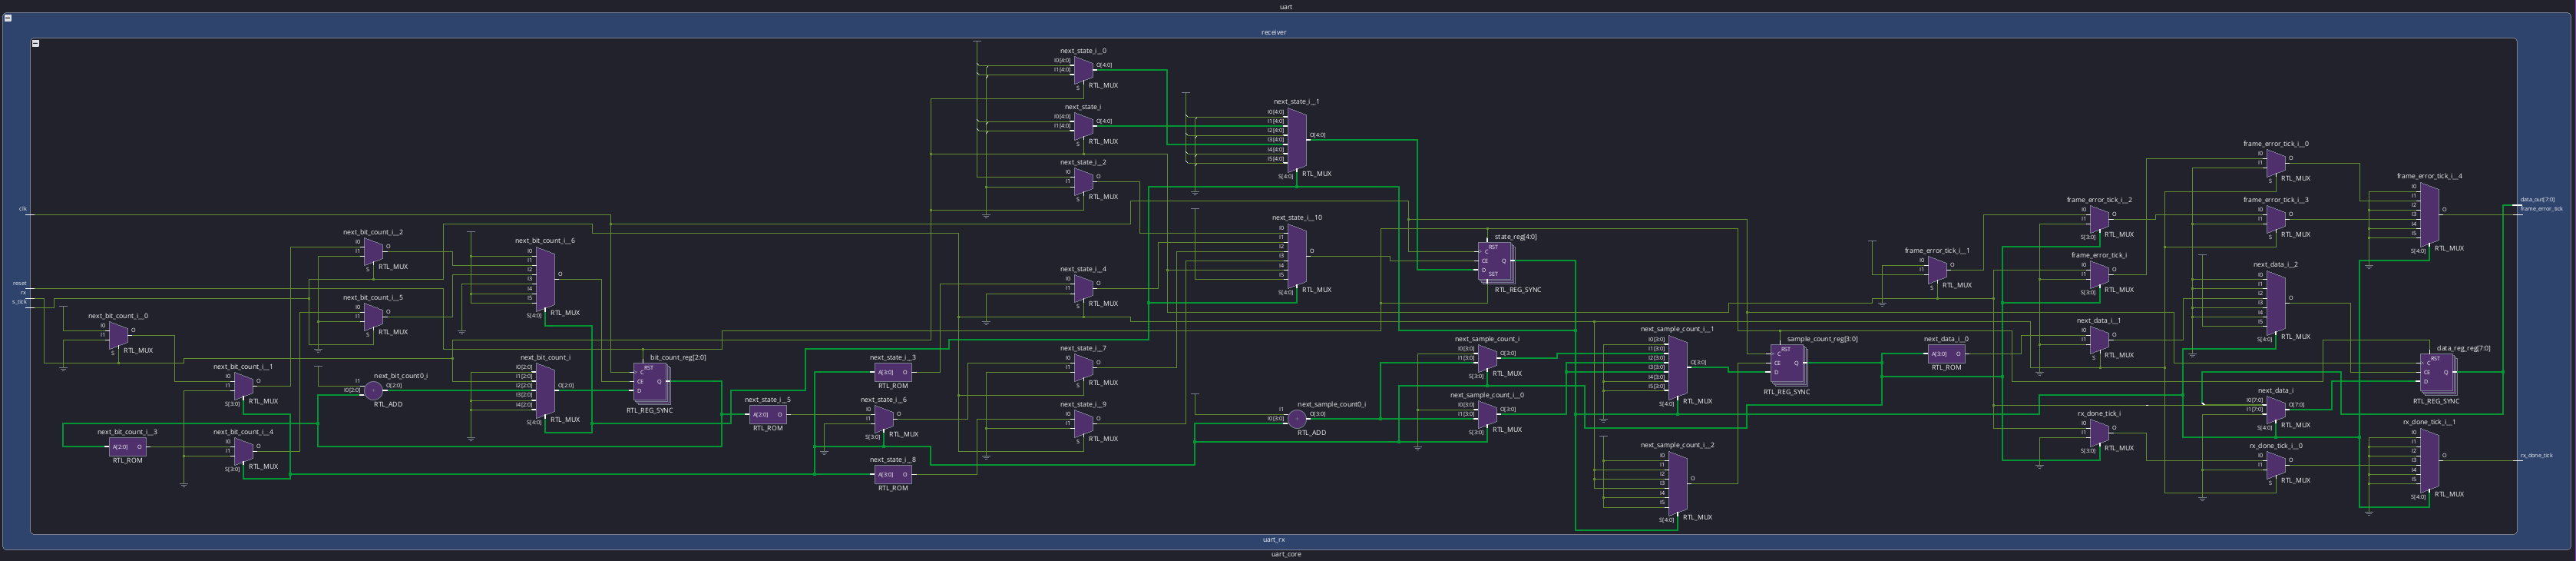
\includegraphics[width=\textwidth]{img/vivado_schematic_uart_rx_rtl.png}
	\vspace{0.6em}

	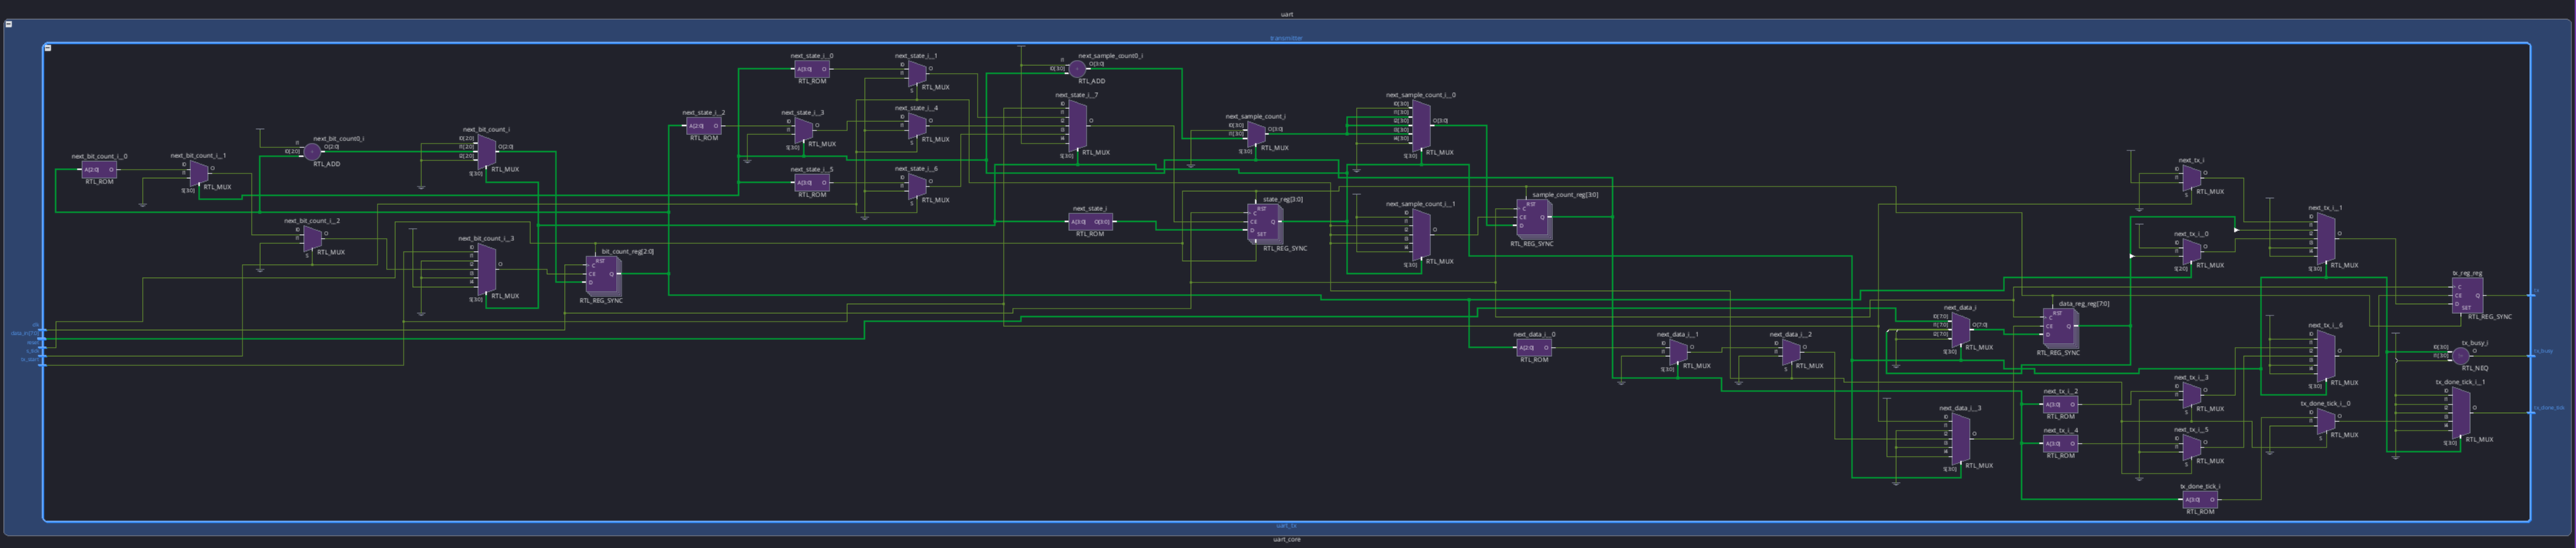
\includegraphics[width=\textwidth]{img/vivado_schematic_uart_tx_rtl.png}
	\caption{Esquemáticos RTL del receptor y del transmisor UART.}%
	\label{fig:schematics-rx-tx-rtl}
\end{figure}

Entre los módulos UART y el controlador se encuentran las dos instancias de
\texttt{fifo}. La figura~\ref{fig:schematics-fifo-rtl} permite comparar la
cola de recepción con la de transmisión. Ambas conservan la misma estructura,
aunque cada una almacena los bytes de un sentido diferente del enlace.

\begin{figure}[H]
	\centering
	\begin{minipage}[t]{0.49\textwidth}
		\centering
		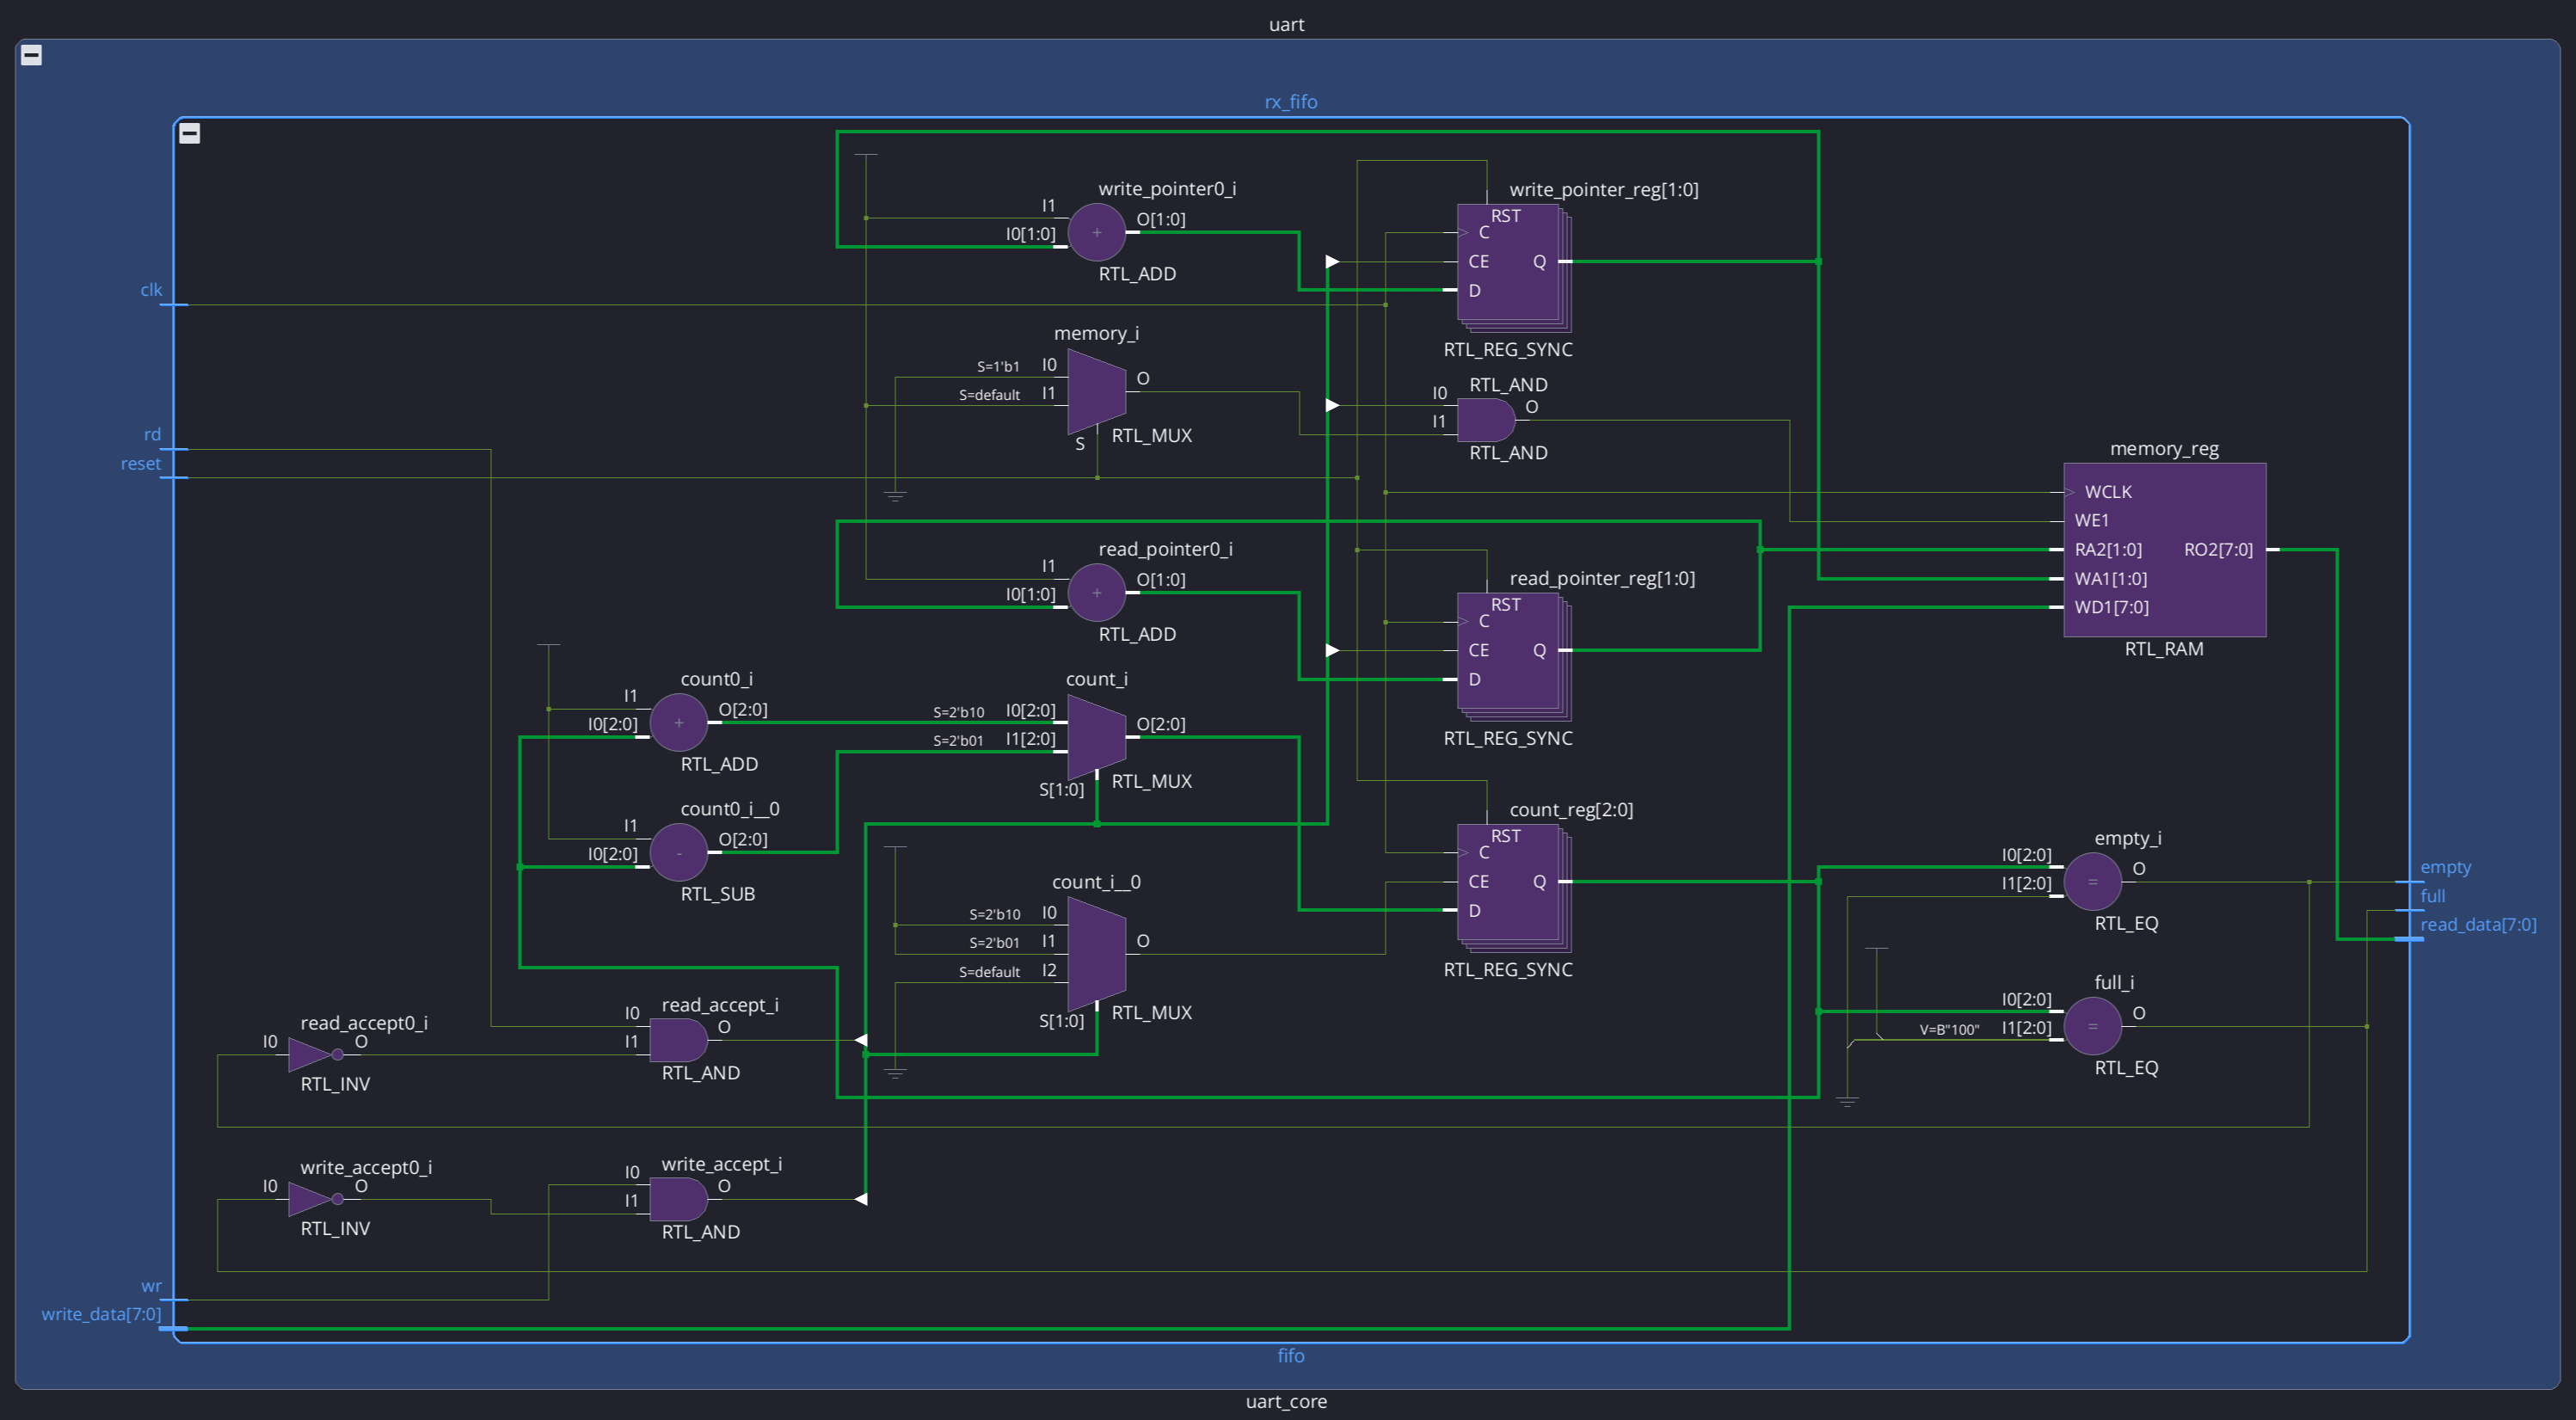
\includegraphics[width=\linewidth]{img/vivado_schematic_rx_fifo_rtl.png}
	\end{minipage}\hfill
	\begin{minipage}[t]{0.49\textwidth}
		\centering
		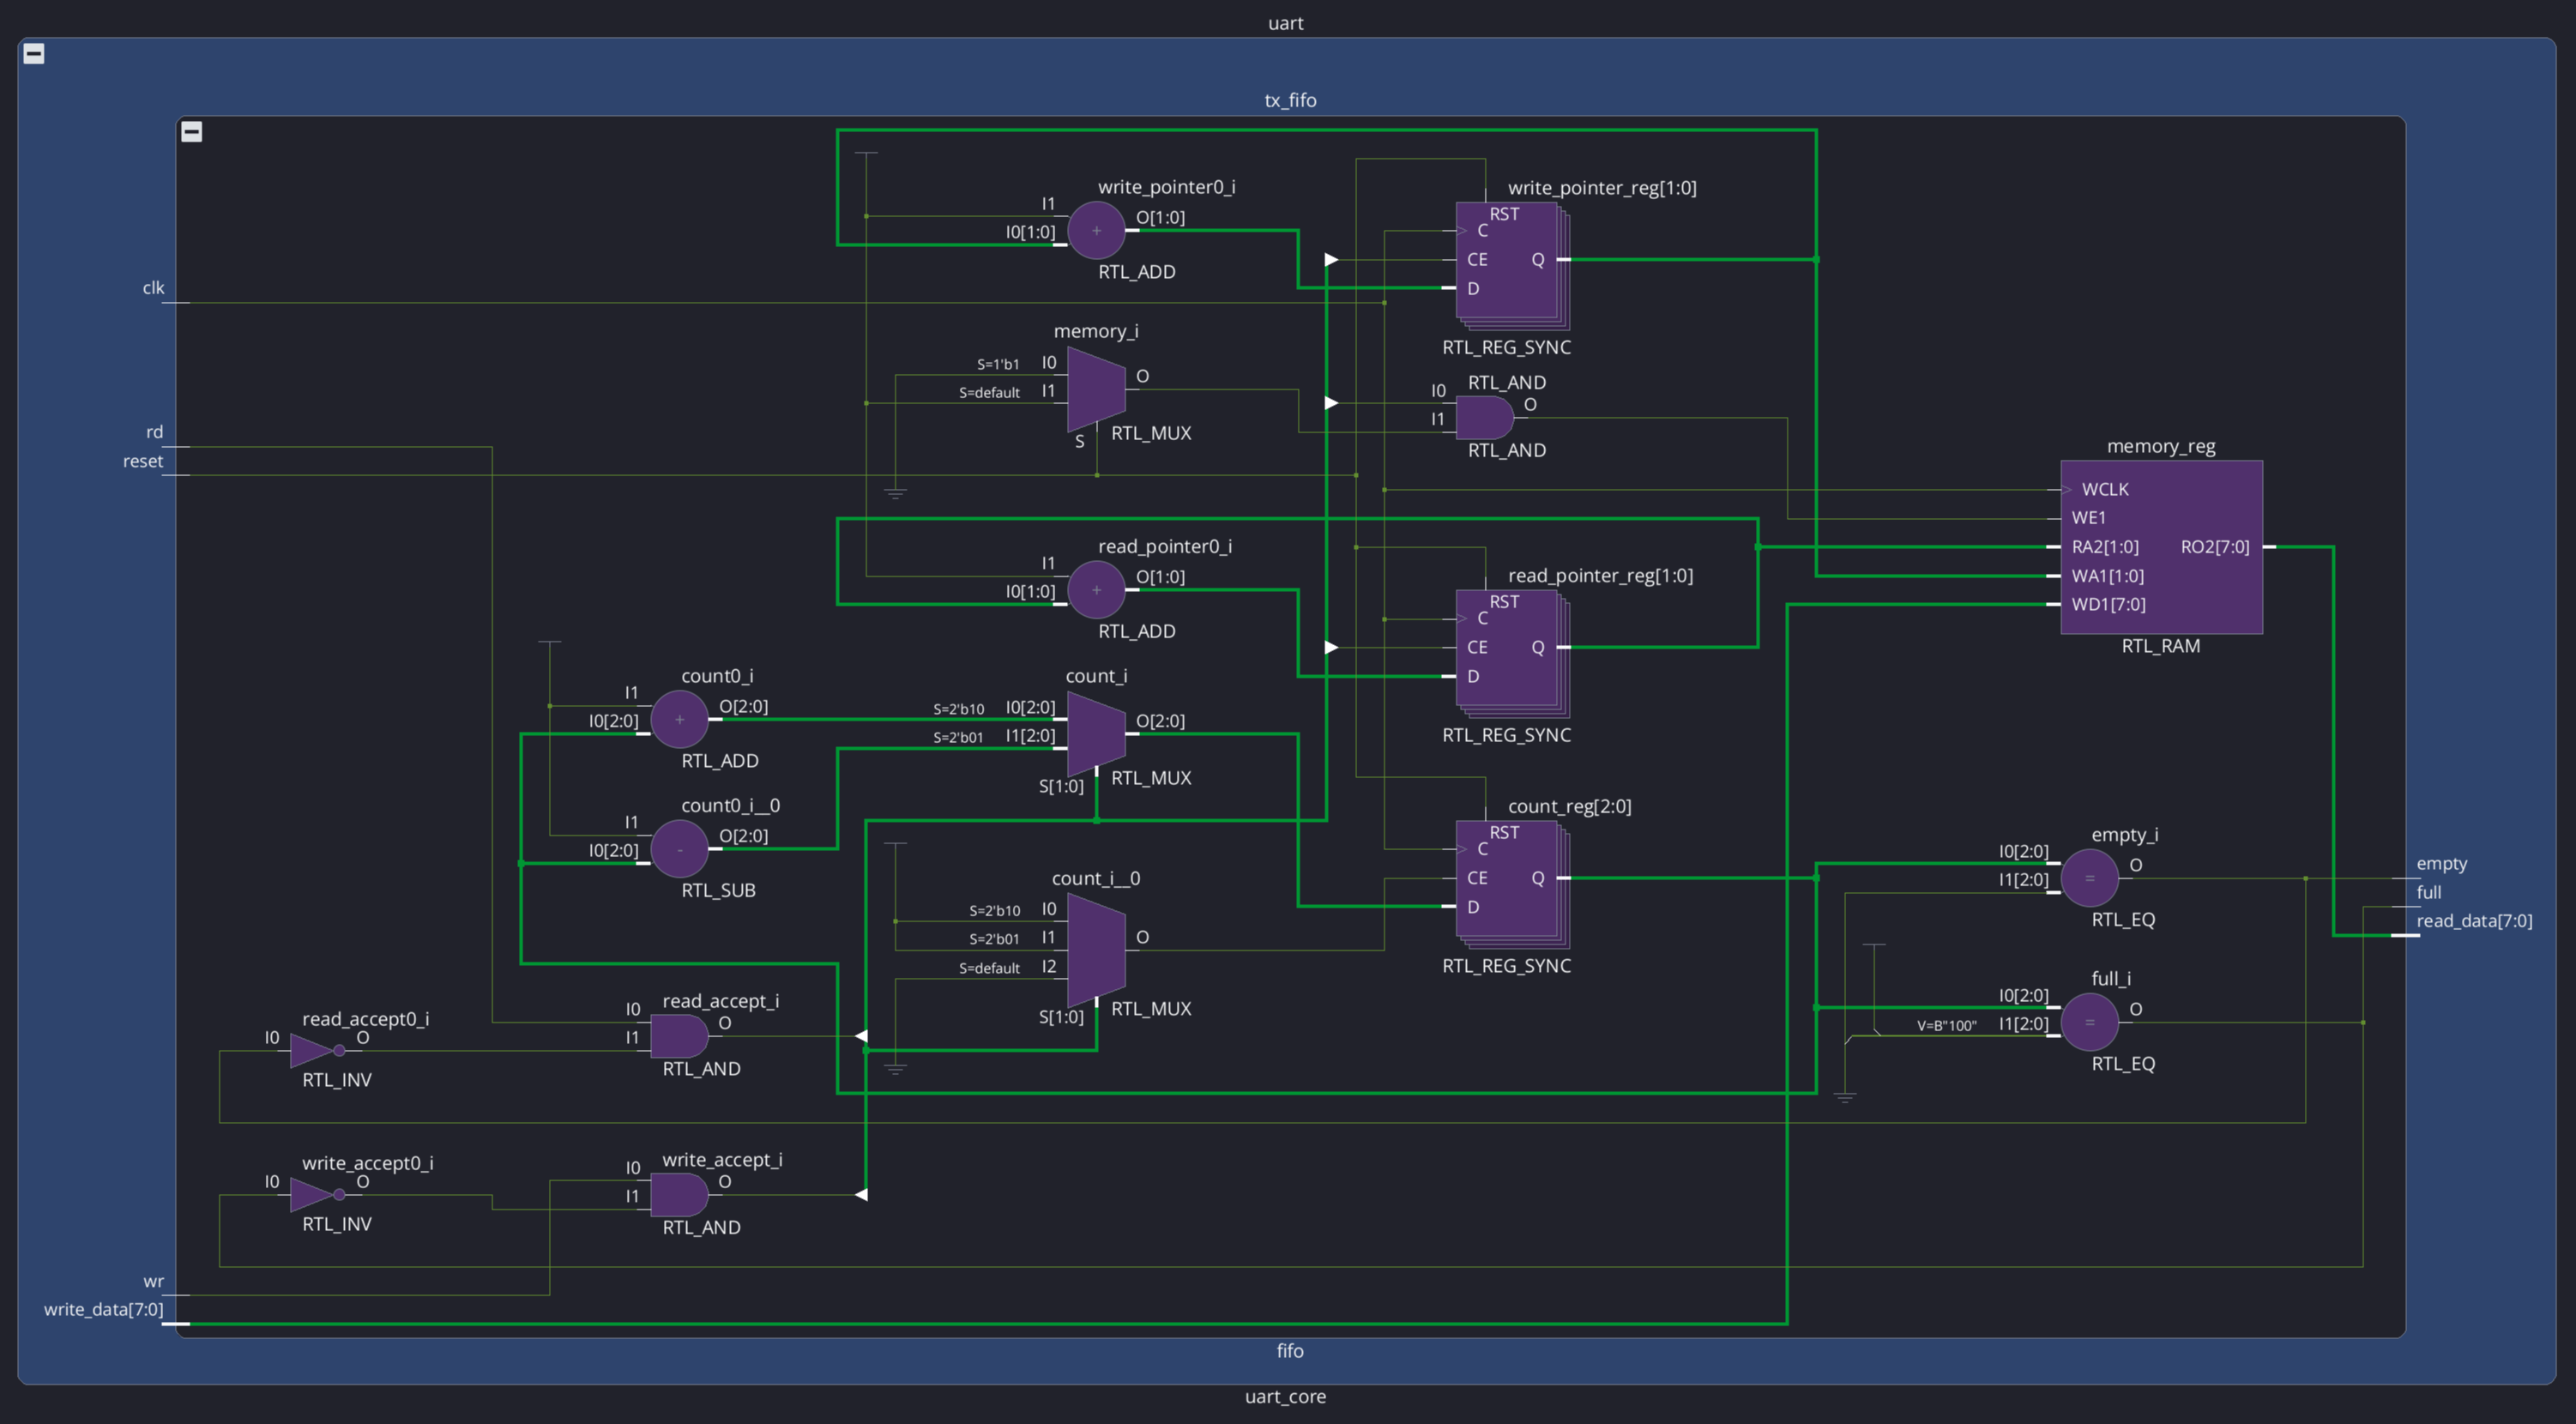
\includegraphics[width=\linewidth]{img/vivado_schematic_tx_fifo_rtl.png}
	\end{minipage}
	\caption{Esquemáticos RTL de las instancias FIFO de recepción y transmisión.}%
	\label{fig:schematics-fifo-rtl}
\end{figure}

Una vez reconstruidos los bytes, el controlador debe interpretar la solicitud y
coordinar la respuesta. La figura~\ref{fig:schematic-controller-rtl} muestra
la estructura elaborada a partir del archivo
\texttt{rtl/alu\allowbreak\_uart\allowbreak\_controller.sv}. En ella se mantienen diferenciados los
registros de la transacción y la lógica que controla su avance.

\begin{figure}[H]
	\centering
	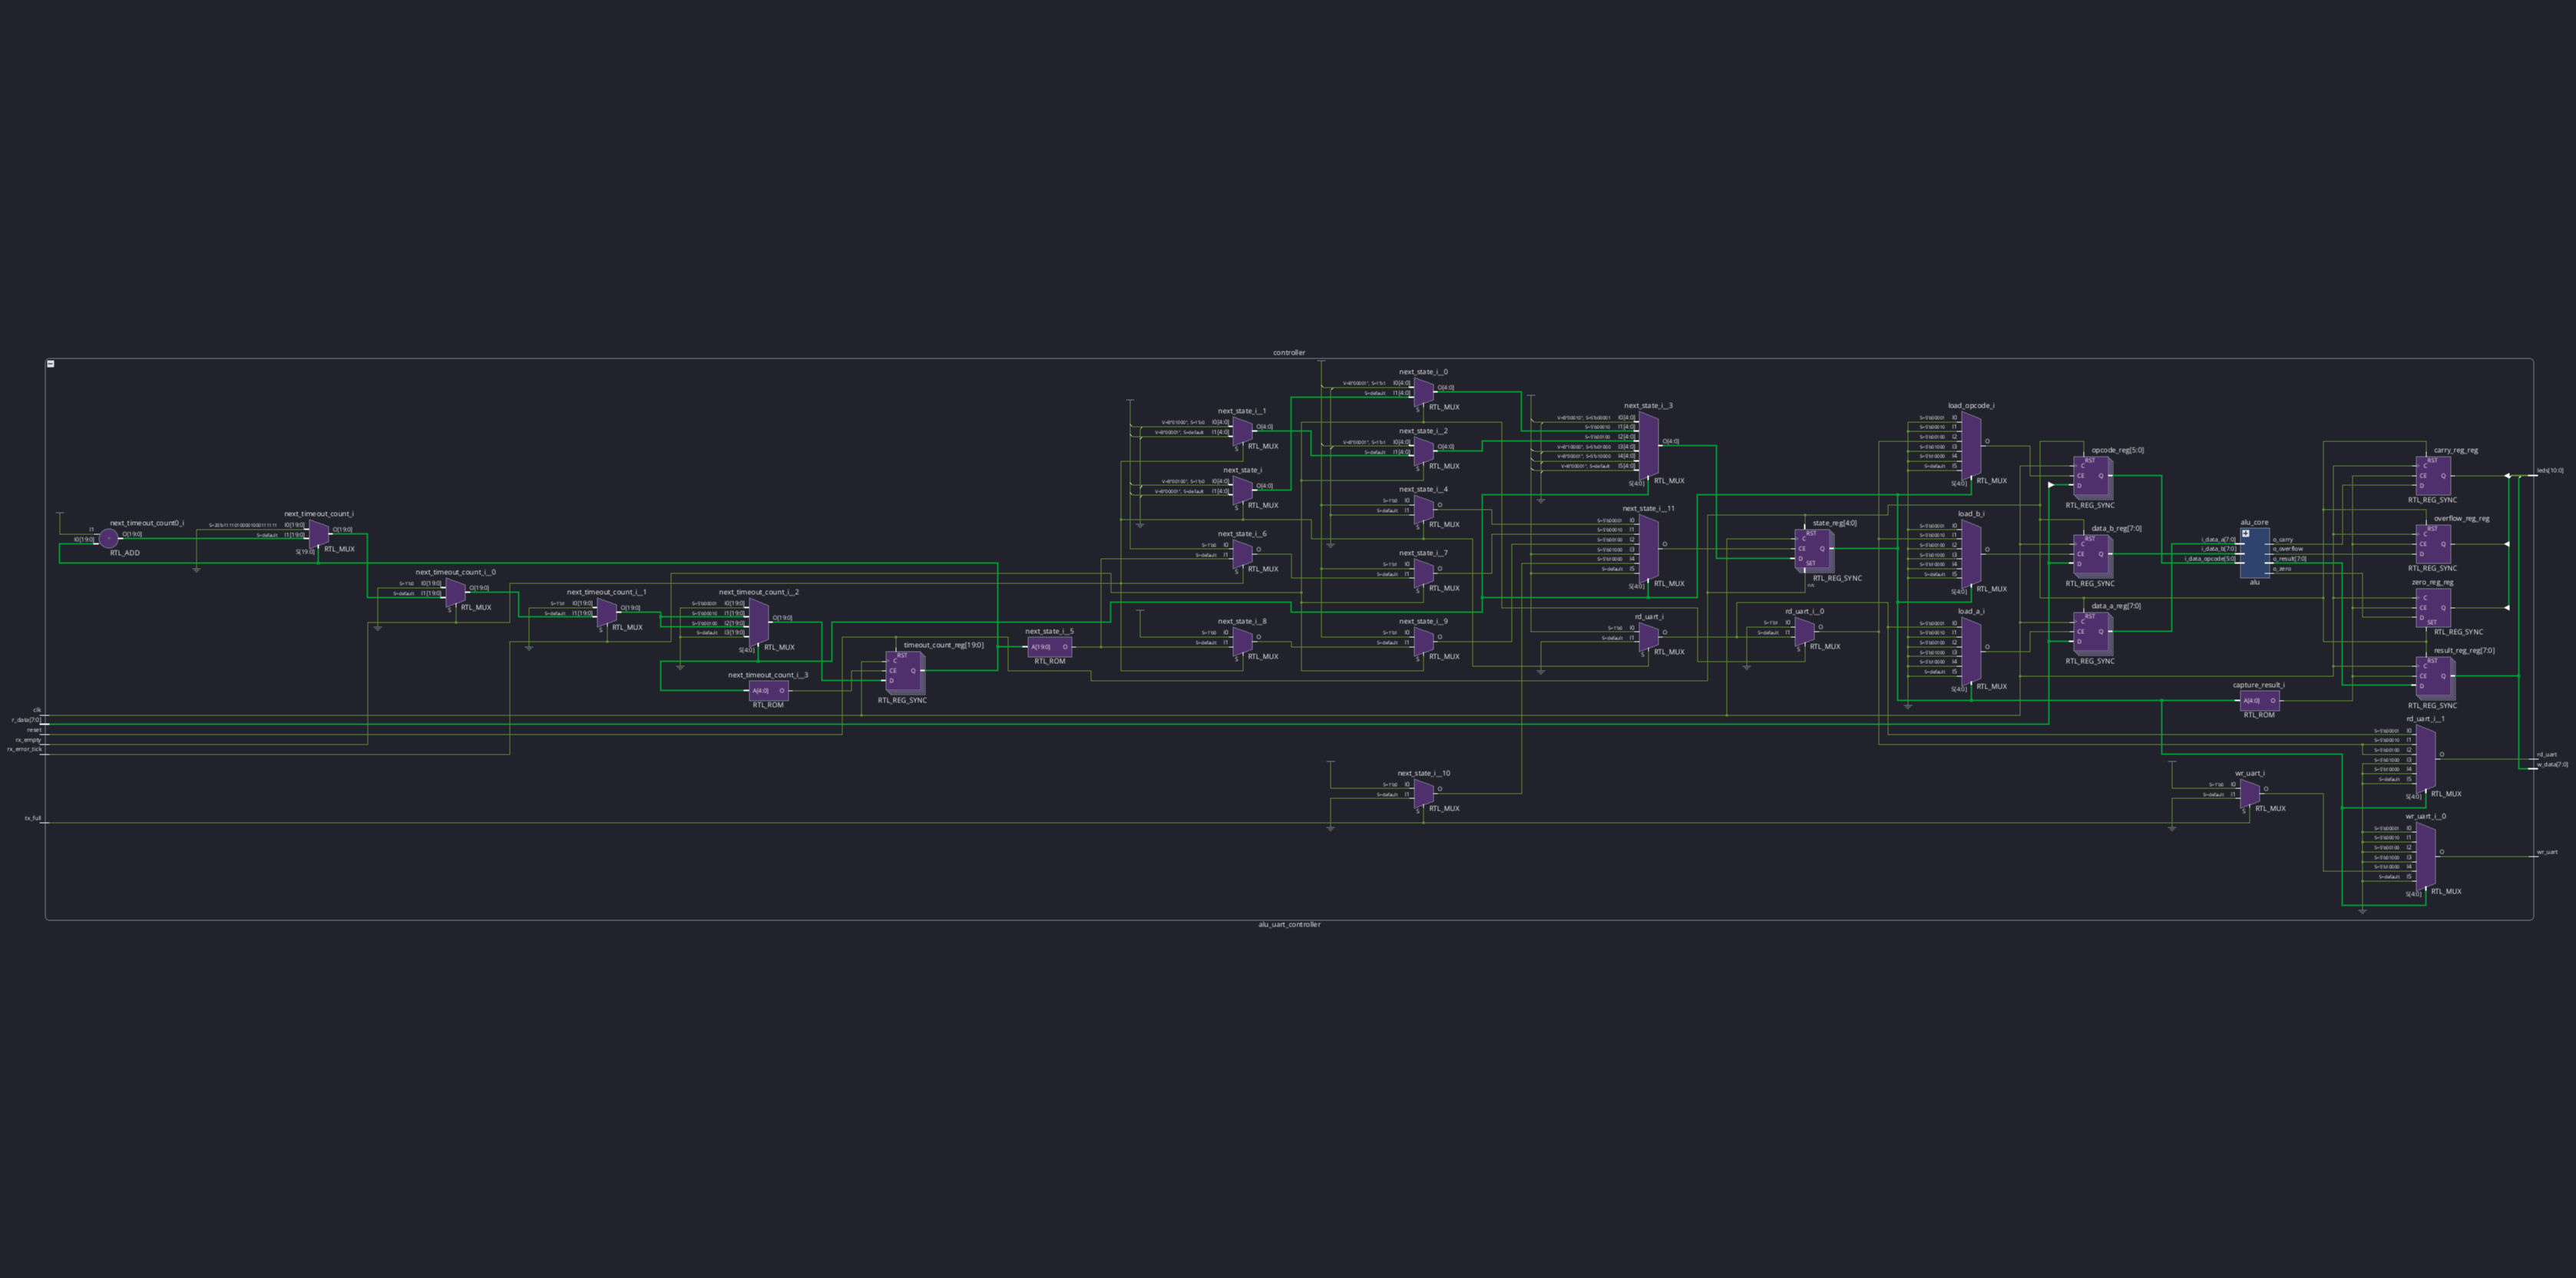
\includegraphics[width=\textwidth]{img/vivado_schematic_controller_rtl.png}
	\caption{Esquemático RTL elaborado del controlador de transacciones.}%
	\label{fig:schematic-controller-rtl}
\end{figure}

La última parte del camino corresponde al cálculo. El esquemático de la
figura~\ref{fig:schematic-alu-rtl} muestra la ALU combinacional elaborada desde
\texttt{rtl/alu.sv}. La ausencia de registros dentro de este bloque coincide
con la decisión de almacenar el resultado y las banderas en el controlador.

\begin{figure}[H]
	\centering
	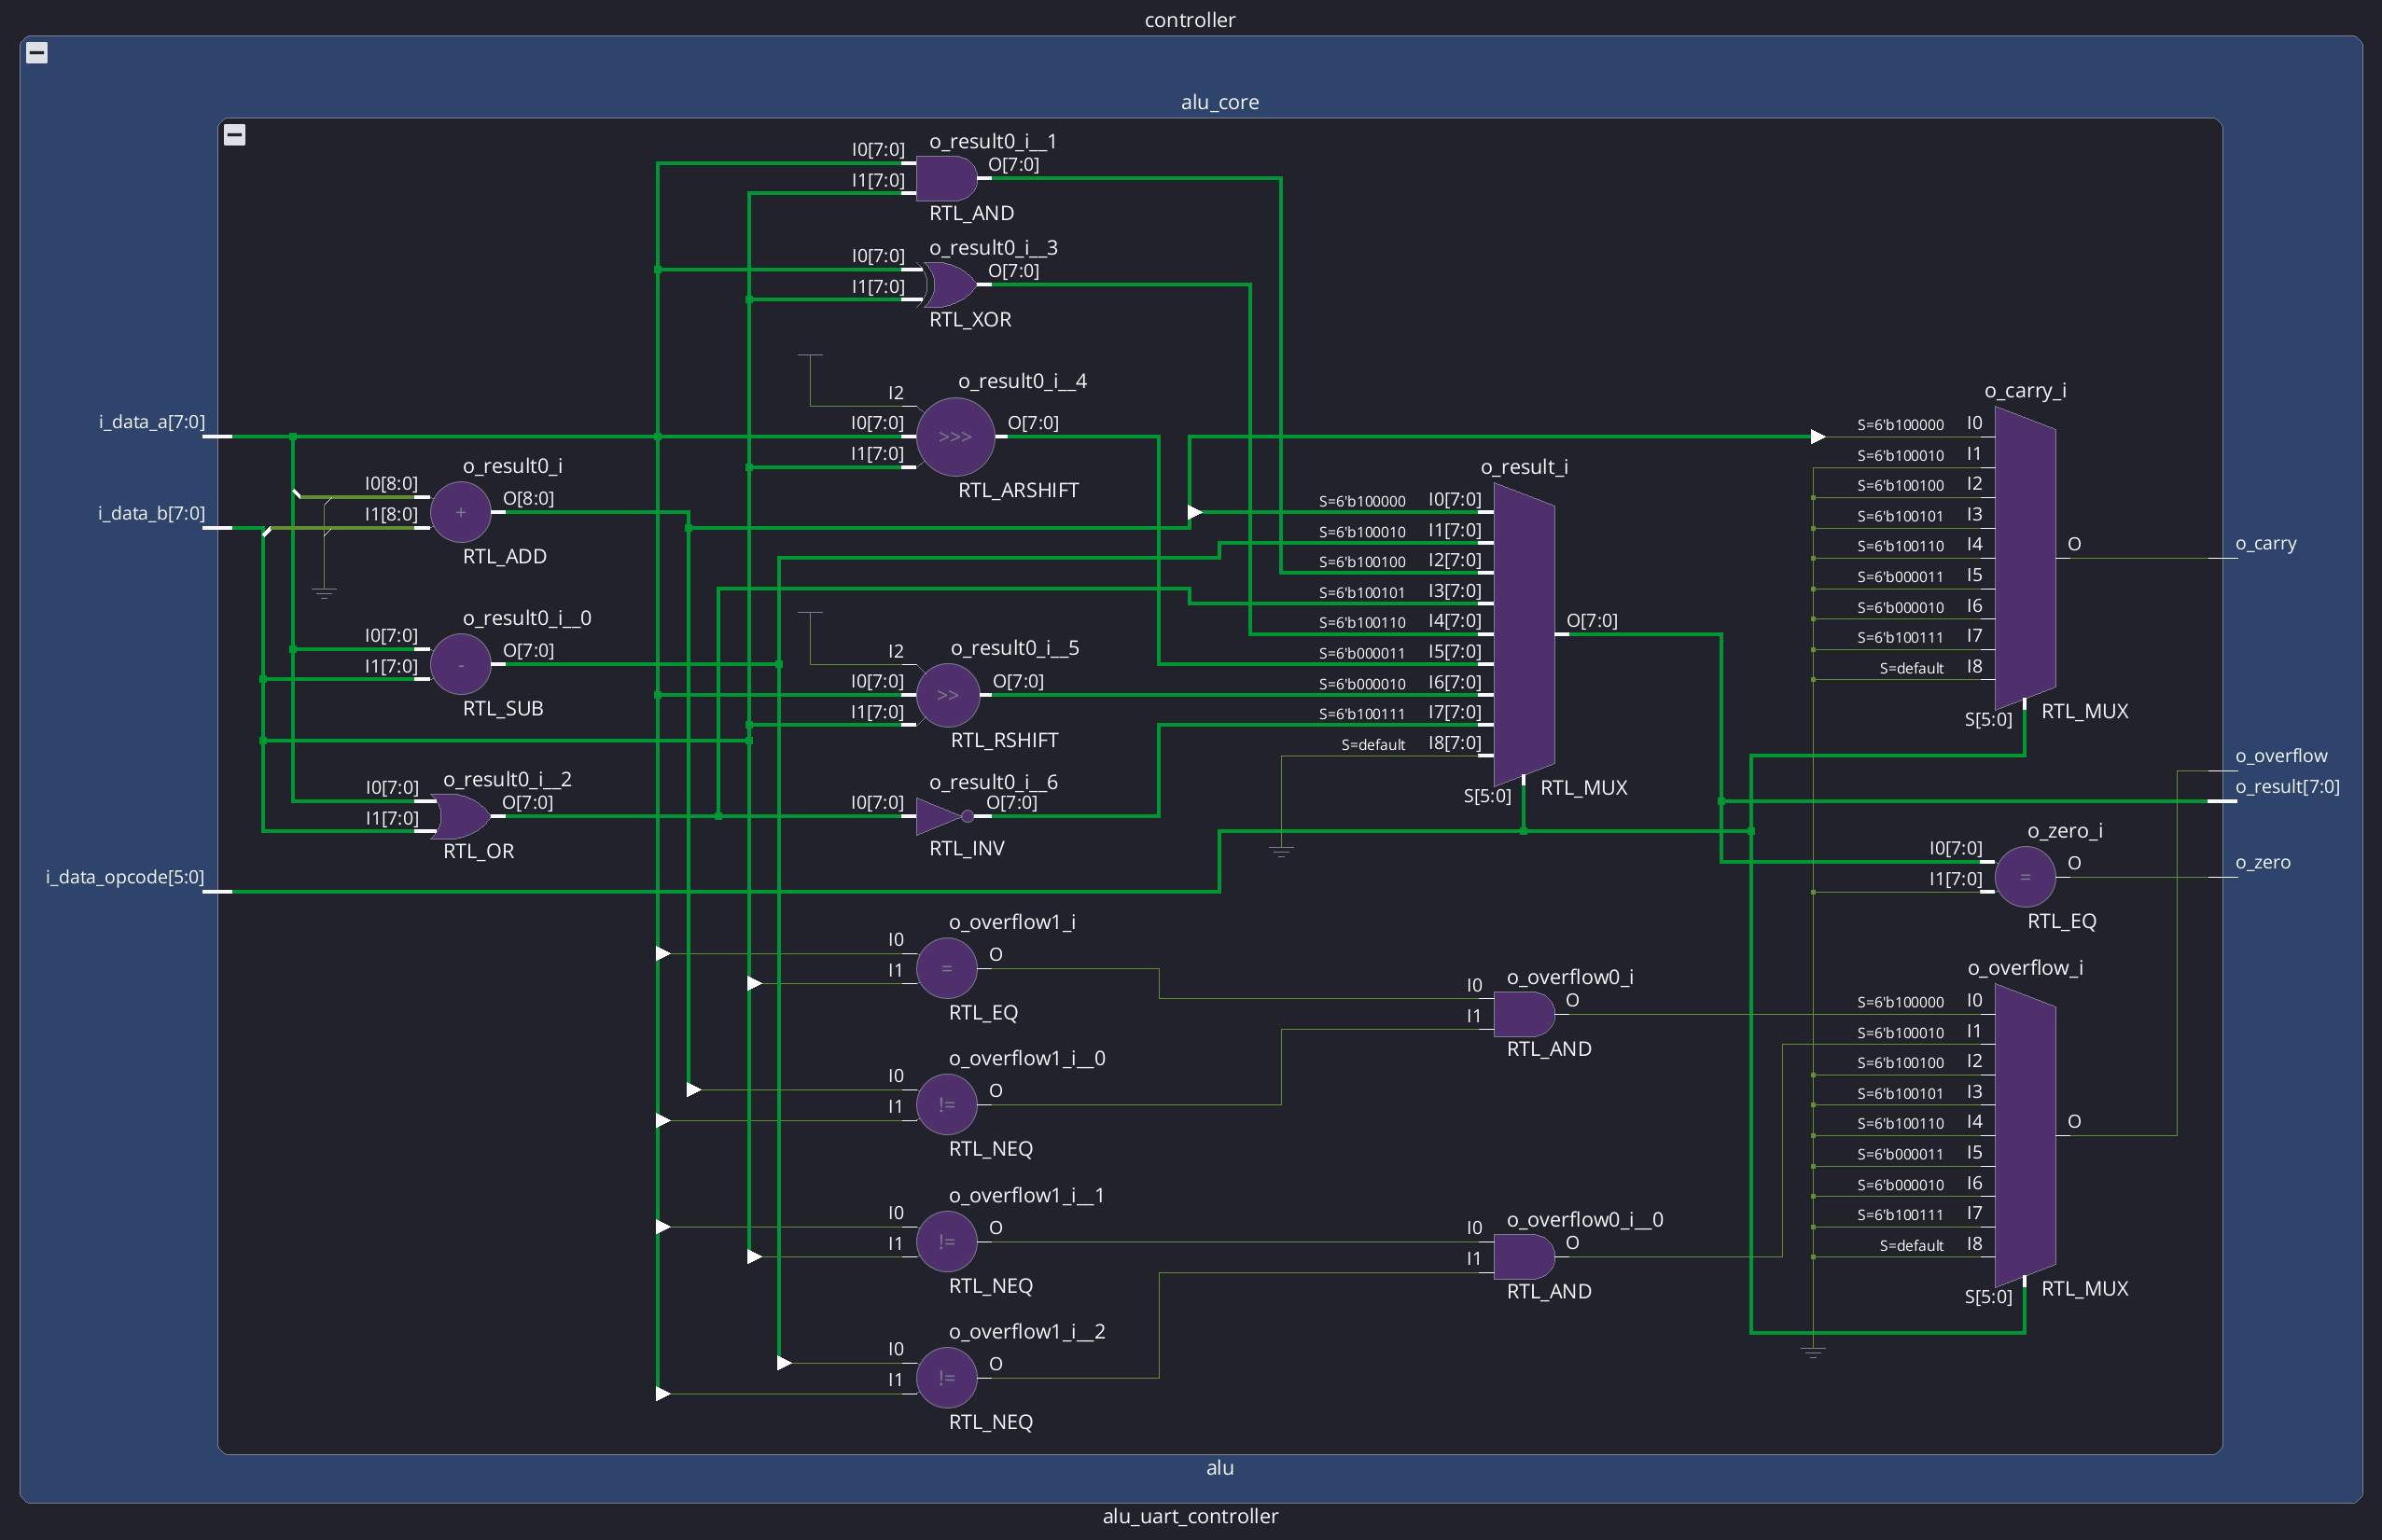
\includegraphics[width=0.78\textwidth]{img/vivado_schematic_alu_rtl.png}
	\caption{Esquemático RTL elaborado de la ALU combinacional.}%
	\label{fig:schematic-alu-rtl}
\end{figure}

En conjunto, estos esquemáticos muestran que la elaboración conservó la
separación prevista entre la comunicación UART, el almacenamiento, el control
de la transacción y el cálculo.

\section{Del esquema RTL a los recursos físicos}

Después de comprobar la jerarquía elaborada, se analizó la forma en que Vivado
la convirtió en recursos del Artix-7. Esta comparación permite determinar si
los registros, las memorias y la lógica combinacional fueron inferidos de
acuerdo con la arquitectura.

Los contadores de sobremuestreo, los índices de bits, el contador del timeout y
los contadores de ocupación necesitan conservar un valor entre ciclos. Por esta
razón aparecen como flip-flops acompañados por las LUT que calculan su próximo
valor.

Las tres máquinas de estado utilizan en total catorce bits. Cinco corresponden
al receptor, cuatro al transmisor y cinco al controlador. Vivado implementa
estos bits con registros y utiliza LUT para determinar las transiciones. Los
catorce bits no representan estados activos al mismo tiempo. Durante el
funcionamiento normal permanece activo un solo bit de cada máquina.

Cada FIFO contiene un arreglo de cuatro palabras de ocho bits. Debido a su
tamaño, no resulta conveniente utilizar un bloque completo de memoria. Vivado
implementa ambos arreglos como memoria distribuida en LUTRAM. Esto explica las
12 LUT utilizadas como memoria después del ruteo y la ausencia de bloques RAM.

La ALU se implementa mediante LUT y cadenas de carry para las operaciones de
suma y resta. No requiere bloques DSP. Los registros de los operandos, del
opcode, del resultado y de las banderas también forman parte de los 134
flip-flops informados. A esos registros se suman los utilizados para los
desplazamientos y los distintos contadores.

La conexión con la placa utiliza tres buffers de entrada. Estos corresponden al
reloj, el reset y la línea RX. También utiliza doce buffers de salida para TX y
los once LED. En total se ocupan 15 IOB.

El reloj que ingresa por el pin W5 utiliza un único BUFG. El generador de baud
no agrega otro buffer global porque \texttt{s\_tick} funciona como una
habilitación síncrona y no como un segundo reloj. Si la implementación hubiera
incorporado una BRAM, un DSP o un segundo BUFG, habría sido necesario revisar
la inferencia realizada por la herramienta.

Los esquemáticos implementados permiten observar esta traducción. A diferencia
de la vista RTL, ya no muestran solamente los módulos descriptos en
SystemVerilog. En ellos aparecen los registros, las LUT, las cadenas de carry y
las conexiones adaptadas al dispositivo después de la colocación y el ruteo.

La figura~\ref{fig:schematic-top-implemented} presenta la vista general del
nivel superior ya implementado.

\begin{figure}[H]
	\centering
	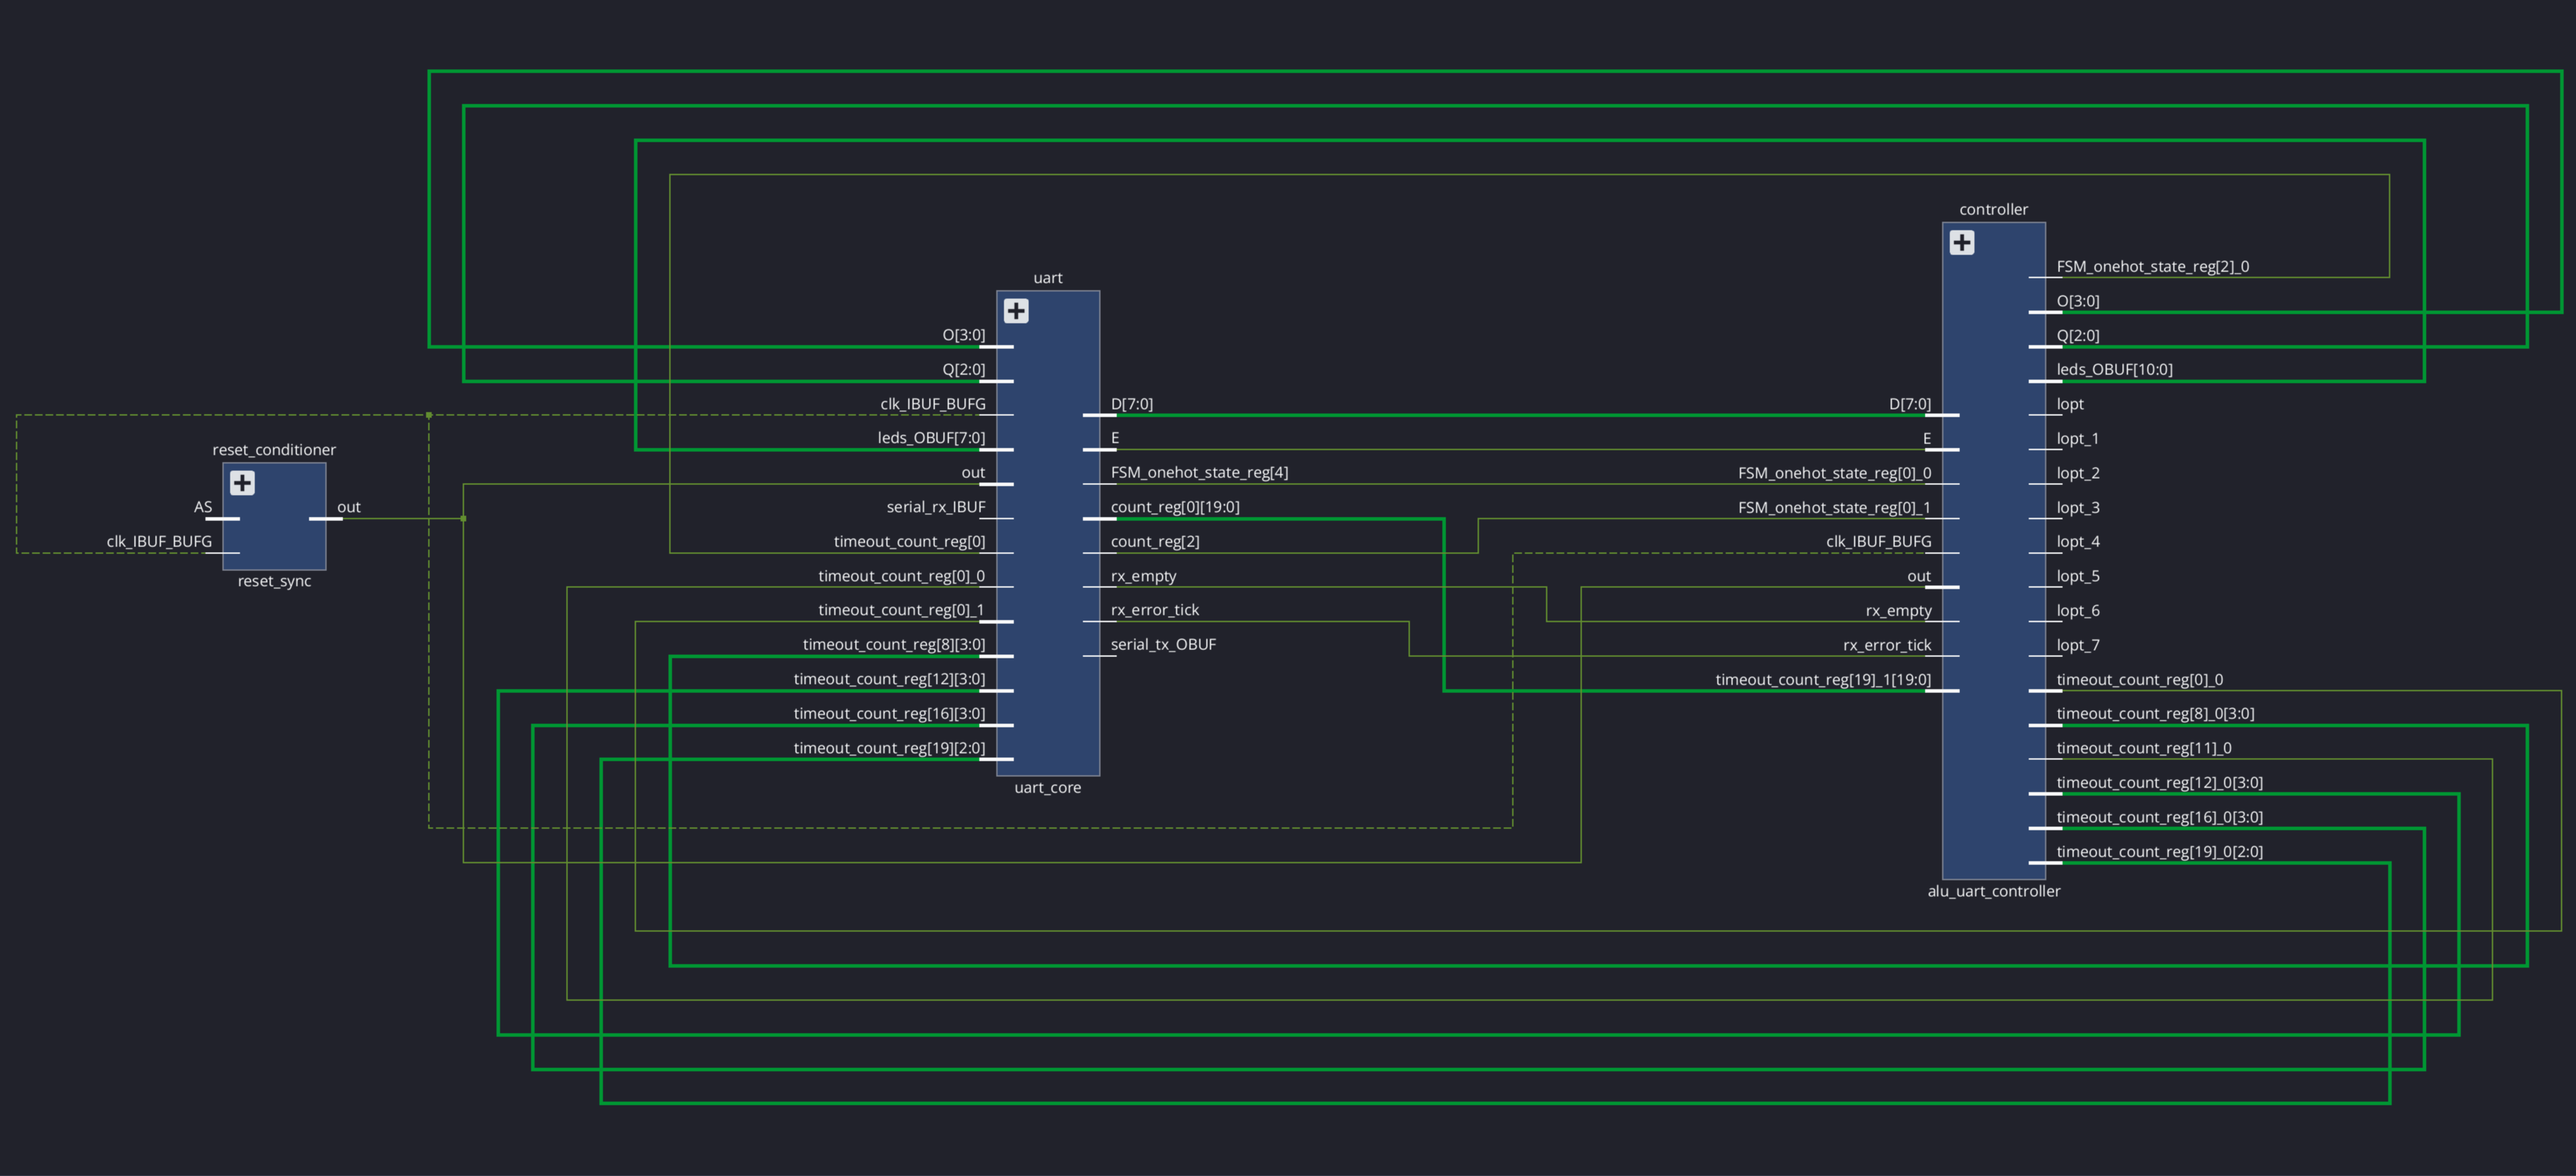
\includegraphics[width=\textwidth]{img/vivado_schematic_top_implementation.png}
	\caption{Esquemático implementado del nivel superior.}%
	\label{fig:schematic-top-implemented}
\end{figure}

Al abrir el núcleo UART se obtiene el esquema de la
figura~\ref{fig:schematic-uart-core-implemented}. En esta vista se observan los
recursos que forman los dos caminos de comunicación y sus conexiones internas.

\begin{figure}[H]
	\centering
	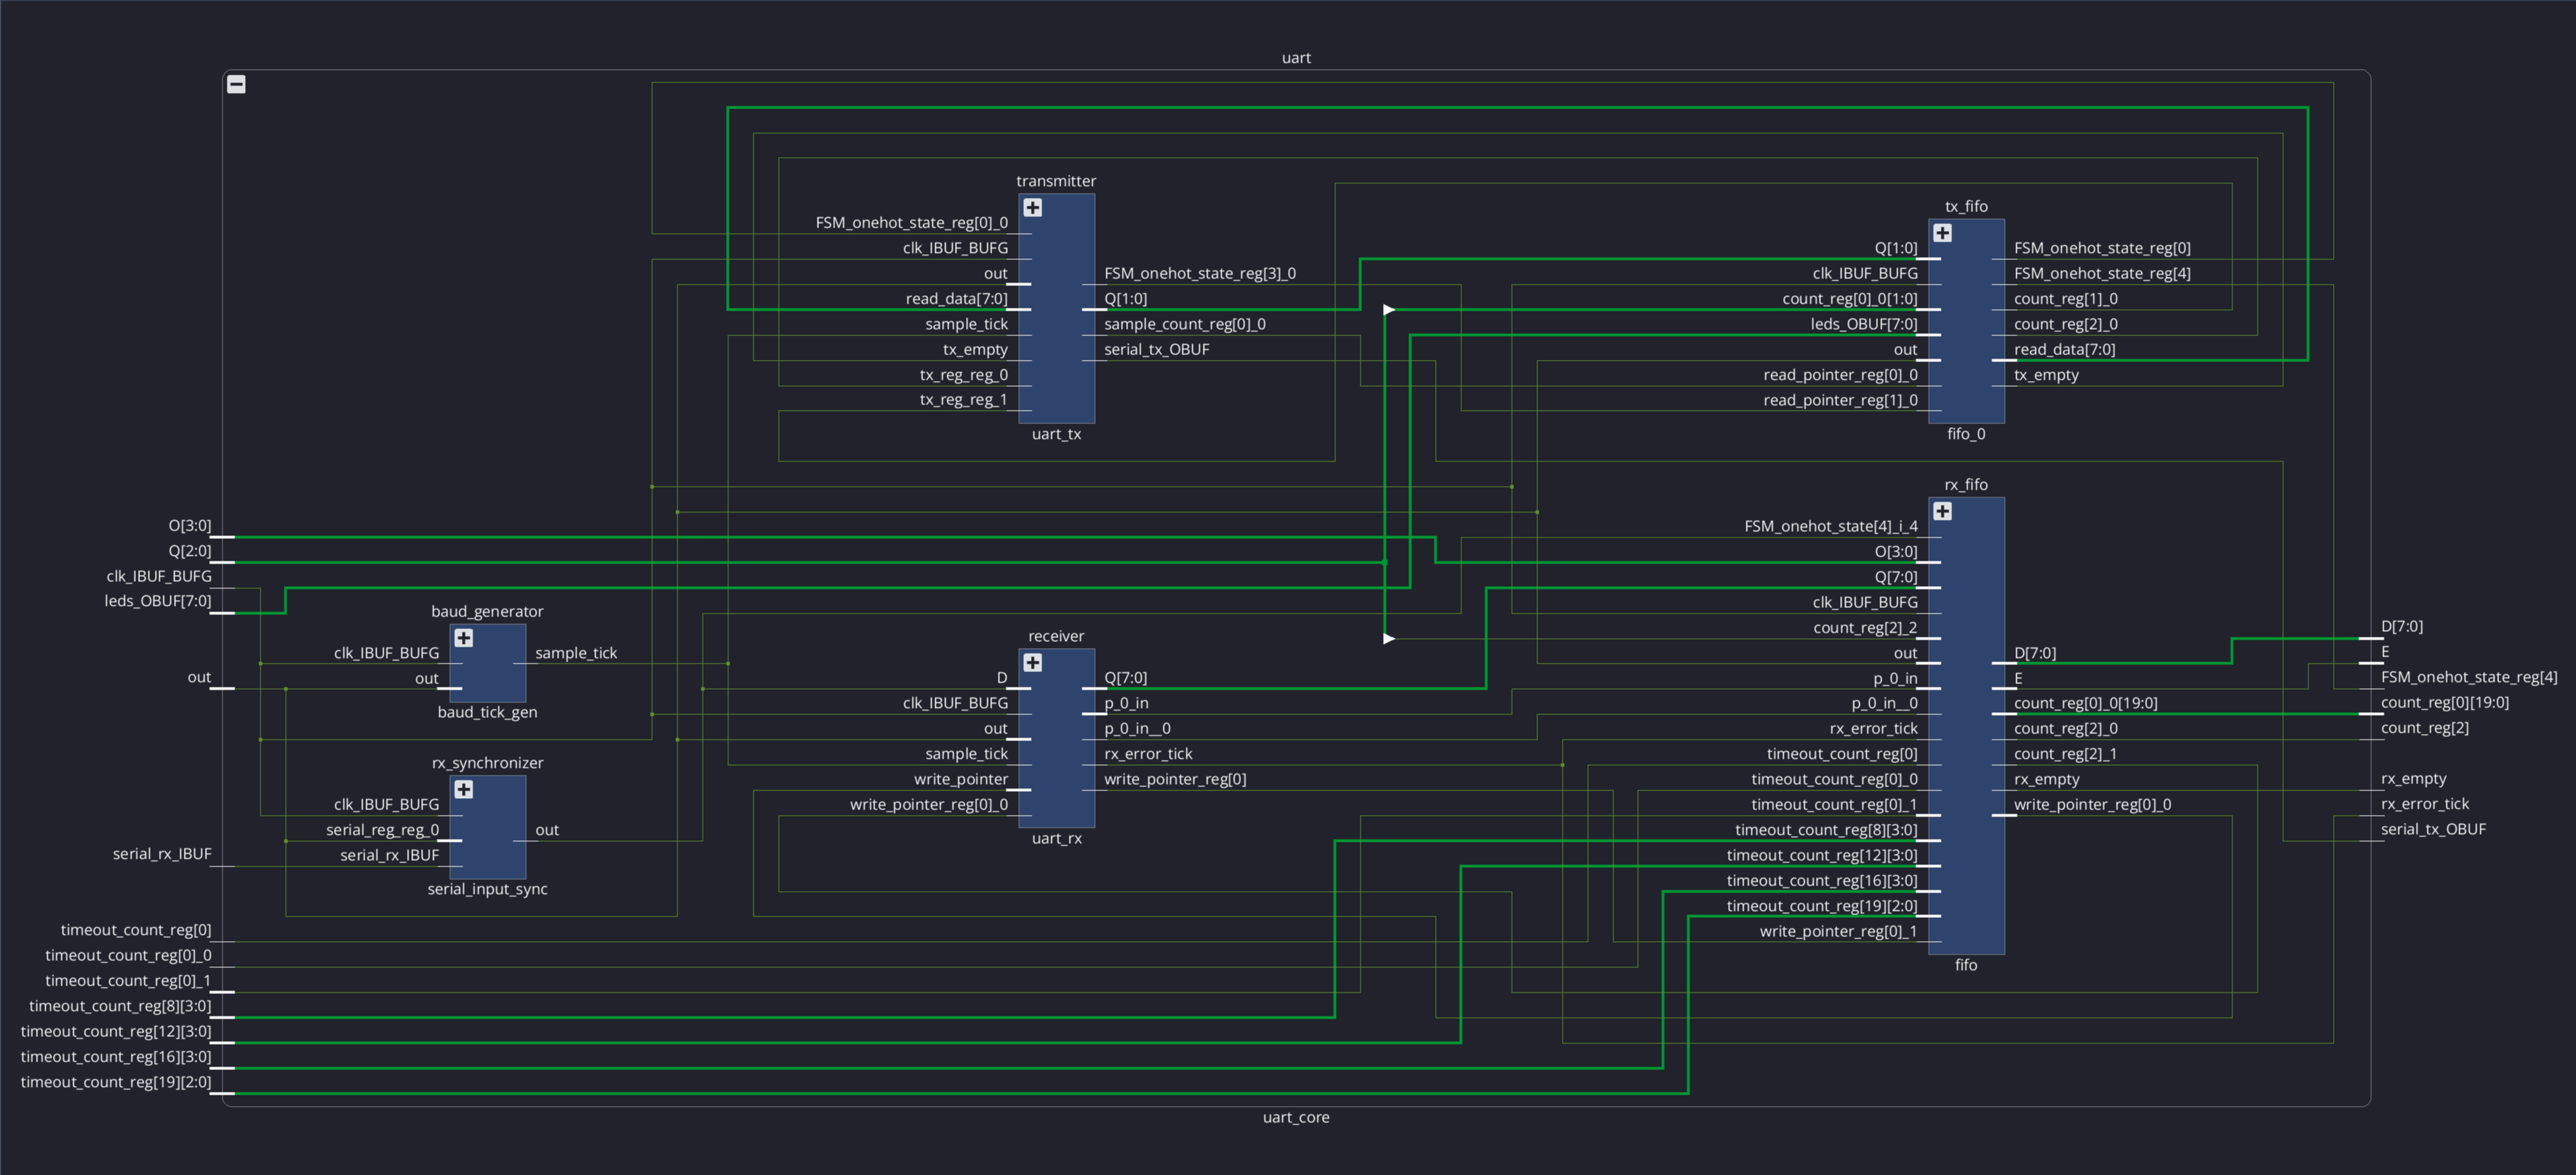
\includegraphics[width=\textwidth]
	{img/vivado_schematic_uart_core_implementation.png}
	\caption{Esquemático implementado del núcleo UART.}%
	\label{fig:schematic-uart-core-implemented}
\end{figure}

La figura~\ref{fig:schematic-controller-implemented} muestra la implementación
del controlador. Los registros que conservan la transacción y las LUT que
determinan las transiciones reemplazan la representación de mayor nivel
observada durante la elaboración.

\begin{figure}[H]
	\centering
	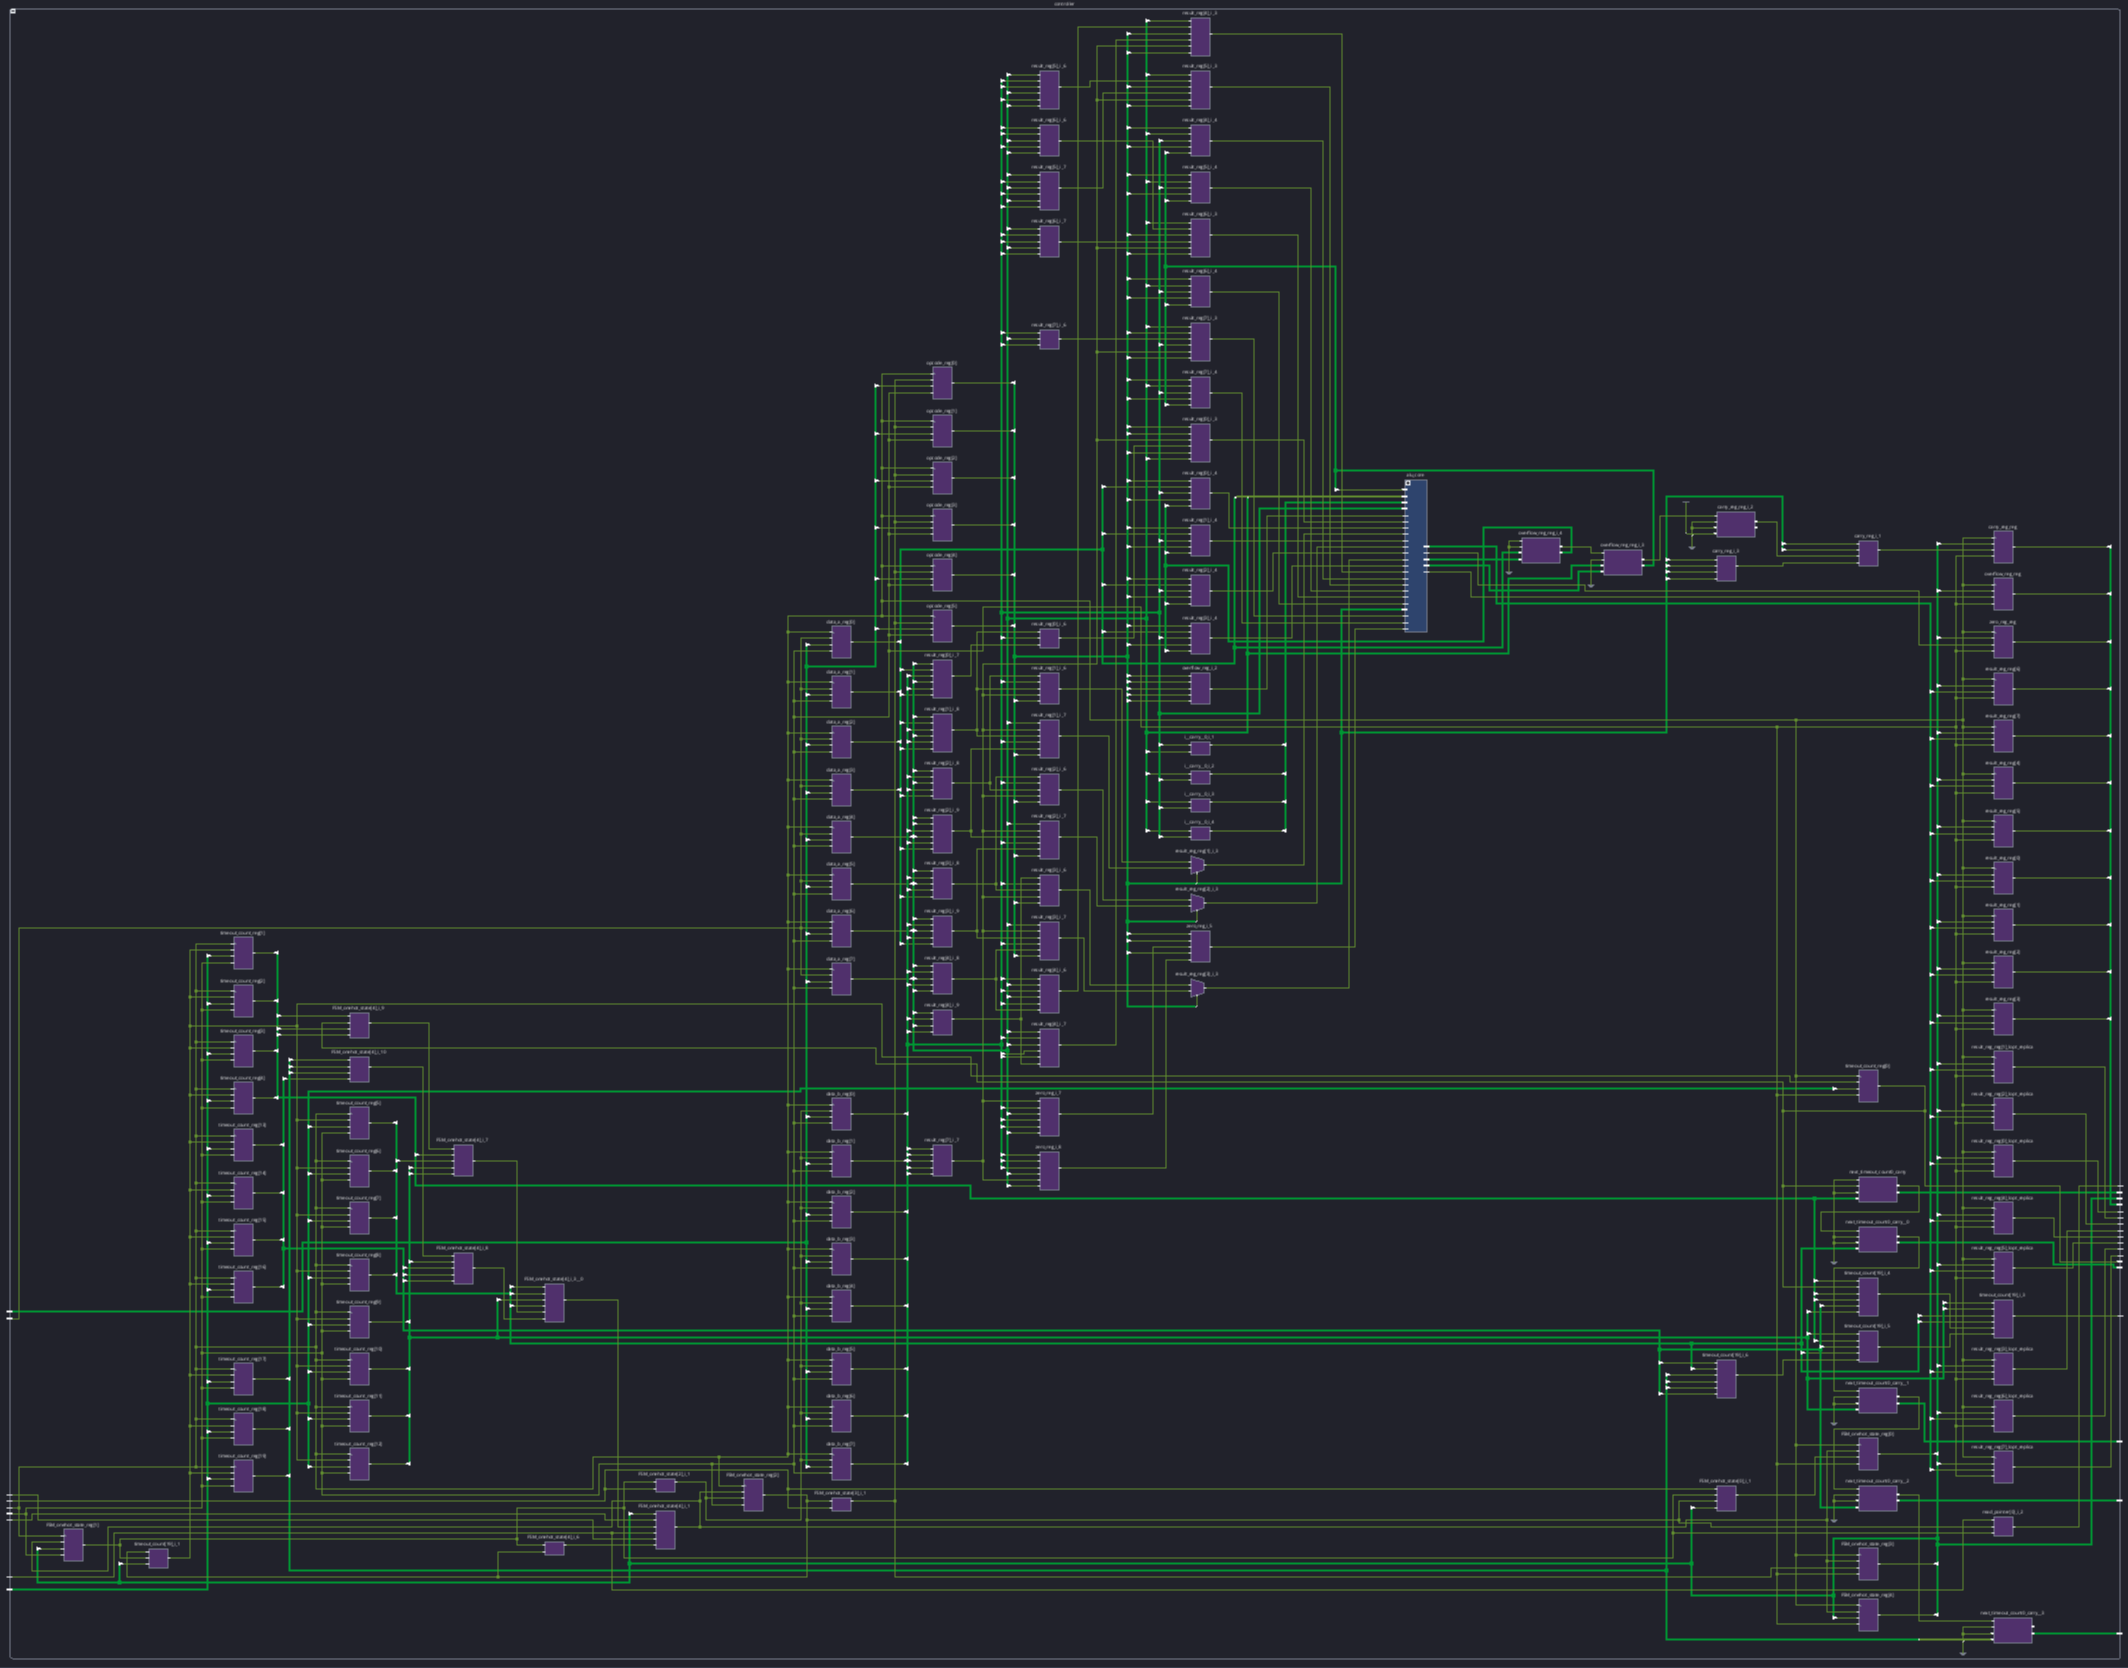
\includegraphics[height=13.0cm,keepaspectratio]
	{img/vivado_schematic_controller_implementation.png}
	\caption{Esquemático implementado del controlador de transacciones.}%
	\label{fig:schematic-controller-implemented}
\end{figure}

Además de los esquemáticos, Vivado permite observar la ubicación de los
recursos sobre el dispositivo. La figura~\ref{fig:device-vivado} muestra que la
lógica ocupa una parte reducida del Artix-7. También permite comprobar que los
pines externos se encuentran en los bancos indicados por las restricciones de
la Basys 3.

\begin{figure}[H]
	\centering
	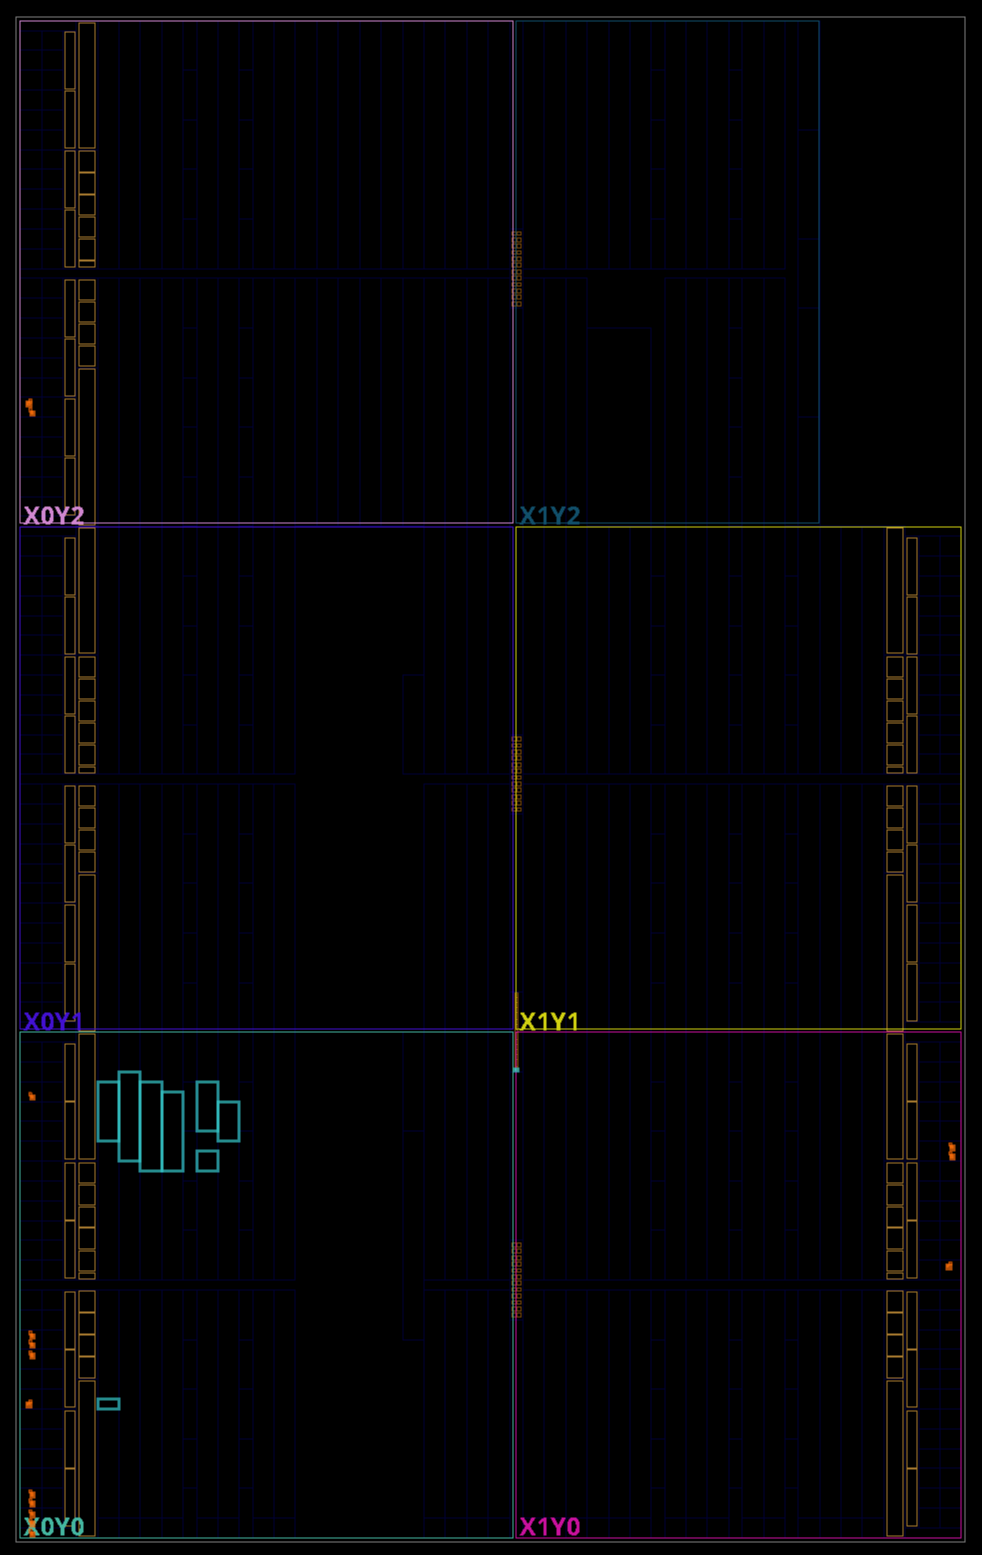
\includegraphics[height=14.5cm,keepaspectratio]{img/vivado_device.png}
	\caption{Vista del dispositivo después de place and route.}%
	\label{fig:device-vivado}
\end{figure}

La tabla~\ref{tab:rtl-recursos} reúne la correspondencia entre los elementos
principales del RTL y los recursos observados después de la implementación.

\begin{table}[H]
	\centering
	\begin{tabularx}{\textwidth}{L{3.5cm}L{4.1cm}Y}
		\toprule
		\textbf{Elemento RTL} & \textbf{Recurso esperado} & \textbf{Observado} \\
		\midrule
		FSM one-hot & Flip-flops y LUT de transición & 14 bits de estado
		dentro de 134 FF. \\
		Dos FIFO $4\times8$ & Memoria distribuida & 12 LUTRAM post-route. \\
		Suma y resta ALU & LUT y carry chain & LUT/MUXF/CARRY4, 0 DSP. \\
		Registros y contadores & Flip-flops & 134 FF, 0 latches. \\
		Reloj de placa & Buffer global & 1 BUFG. \\
		Puertos físicos & IBUF/OBUF e IOB & 15 IOB asignados. \\
		\bottomrule
	\end{tabularx}
	\caption{Correspondencia entre la descripción y los recursos implementados.}%
	\label{tab:rtl-recursos}
\end{table}

\section{Utilización de recursos}

La correspondencia anterior explica qué tipo de recurso se utilizó. Para
conocer cuánto espacio ocupa el diseño, se revisaron los reportes
\texttt{reports/synthesis\_utilization\_summary.rpt} y
\texttt{reports/implementation\_utilization\_summary.rpt}. El primero
corresponde a la salida de la síntesis. El segundo contiene los valores
obtenidos después de la colocación y el ruteo.

La figura~\ref{fig:utilization-summary} presenta el resumen posterior al ruteo.
La figura~\ref{fig:utilization-hierarchy} distribuye esos mismos recursos entre
las instancias del diseño.

\begin{figure}[H]
	\centering
	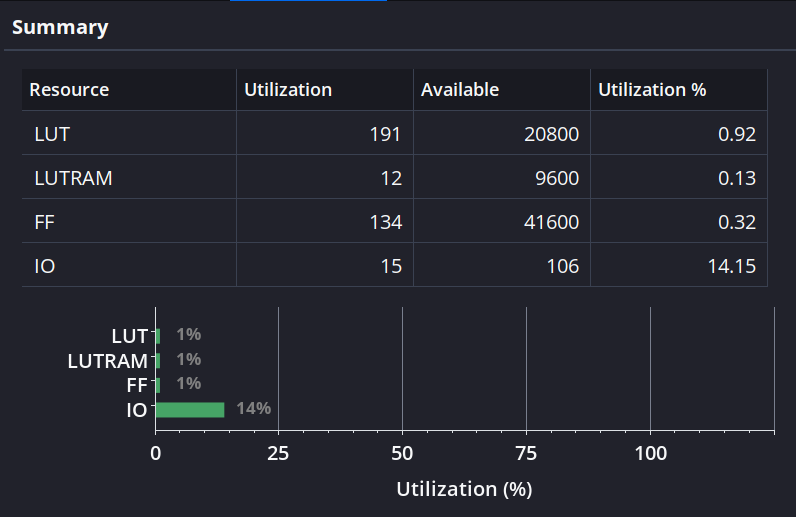
\includegraphics[width=0.65\textwidth]{img/vivado_utilization_summary.png}
	\caption{Resumen de utilización posterior al ruteo.}%
	\label{fig:utilization-summary}
\end{figure}

\begin{figure}[H]
	\centering
	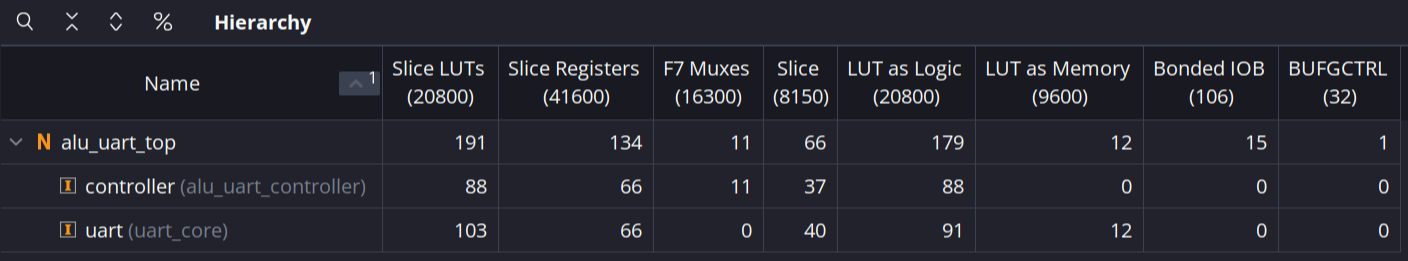
\includegraphics[width=\textwidth]{img/vivado_utilization_hierarchy.png}
	\caption{Distribución jerárquica de los recursos implementados.}%
	\label{fig:utilization-hierarchy}
\end{figure}

Para observar los cambios introducidos durante la implementación, la
tabla~\ref{tab:utilizacion-vivado} compara los valores de síntesis con los
valores posteriores al ruteo.

\begin{table}[H]
	\centering
	\begin{tabularx}{0.88\textwidth}{L{3.2cm}ZZZZ}
		\toprule
		\textbf{Etapa} & \textbf{LUT} & \textbf{LUT lógica} &
		\textbf{LUTRAM} & \textbf{FF} \\
		\midrule
		Síntesis & 197 & 181 & 16 & 126 \\
		Post-route & 191 & 179 & 12 & 134 \\
		Disponible & 20800 & 20800 & 9600 & 41600 \\
		Uso post-route & \SI{0.92}{\percent} & \SI{0.86}{\percent} &
		\SI{0.13}{\percent} & \SI{0.32}{\percent} \\
		\bottomrule
	\end{tabularx}
	\caption{Utilización obtenida antes y después de la implementación.}%
	\label{tab:utilizacion-vivado}
\end{table}

La cantidad total de LUT disminuye de 197 a 191. Dentro de ese total, las LUT
destinadas a lógica pasan de 181 a 179 y las utilizadas como memoria se reducen
de 16 a 12. Estas variaciones se producen durante las optimizaciones físicas de
la implementación.

La cantidad de flip-flops aumenta de 126 a 134. Los ocho registros adicionales
aparecen al adaptar la red sintetizada a los recursos del dispositivo. Tanto la
reducción de LUT como el aumento de registros son pequeños frente a la
capacidad disponible.

El diseño final utiliza 66 slices, 15 de los 106 IOB y uno de los 32 BUFG. No
utiliza BRAM ni DSP. La ocupación de LUT y flip-flops permanece por debajo del
uno por ciento. Estos valores muestran que las dos colas y las tres máquinas de
estado poseen un costo reducido dentro del Artix-7. La ampliación del protocolo
queda fuera del alcance de este trabajo.
